\chapter{From Waves to Wavefunctions}\label{ch:schrodinger}

\begin{chapterintro}
Pluck a guitar string and you hear a definite note, together with a few overtones at two, three, four times its frequency. You do not hear a smear of every possible pitch, because the string is pinned at both ends and only waves that fit between the pins survive. Heat a gas of hydrogen and it glows in a few sharp colors, not in a continuous rainbow. Early in the twentieth century physicists realized that these two facts are cousins: an electron bound in an atom behaves like a wave confined to a region, and only certain wave patterns, with certain energies, fit. The set of allowed energies is called the \emph{spectrum} of the system.

This chapter builds the mathematics of that idea from what you already know about waves on strings. We meet the de Broglie relation that assigns a wavelength to a particle, construct (by motivated guessing, which is honestly all anyone can do) the Schr\"odinger equation, separate it into a time part and a space part, and arrive at the eigenvalue equation $H\psi=E\psi$. We learn what the wavefunction $\psi$ means (the Born rule), how to compute averages of measured quantities, why the operators of quantum mechanics must be \emph{Hermitian} (self-adjoint; a property defined precisely in Sec.~\ref{sec:schrodinger-hermitian}), and why that guarantees real energies. Finally we adopt the units $\hbar=2m=1$ that the paper uses throughout.

Where this shows up in the paper: the very first sentence of the paper speaks of ``the spectrum of a self-adjoint operator''; Sec.~II~B of the paper writes ``In units $\hbar=2m=1$, $H=-d^2/dx^2+V(x)$''; Sec.~II~C works with eigenpairs $(E_n,\psi_n)$ and weights $|\psi_n|^2$; and Secs.~II~E and~V deliberately break Hermiticity with $H\to H+iA$. After this chapter each of those phrases will be a precise statement you can check.
\end{chapterintro}

\begin{prerequisites}
\item First-year physics: traveling waves $y=y_m\sin(kx-\omega t)$, wave speed, the wave equation for a string, standing waves and harmonics on a string fixed at both ends; kinetic energy $K=\tfrac12mv^2=p^2/2m$; the electron-volt.
\item Calculus: derivatives, the chain and product rules, integration by parts, integrals of $\sin^2$ and of exponentials.
\item Chapter~\ref{ch:complex}: complex numbers, modulus $\abs{z}$, complex conjugate $z^*$, Euler's formula $e^{i\theta}=\cos\theta+i\sin\theta$, $\abs{e^{i\theta}}=1$.
\item Chapter~\ref{ch:fourier-series}: superposition, beats, orthogonality of sines and cosines, expanding a function in a series of sines.
\item Chapter~\ref{ch:linear-algebra}: inner products $\int f^*g\,\dd x$ of functions, orthonormal bases.
\item Chapter~\ref{ch:eigen}: eigenvalues and eigenvectors, symmetric and Hermitian matrices have real eigenvalues and orthogonal eigenvectors, the second-derivative operator as a tridiagonal matrix, the fixed-end string problem $-y''=\lambda y$ on $[-L,L]$ with eigenvalues $(k\pi/2L)^2$.
\end{prerequisites}

%======================================================================
\section{Waves you already know}\label{sec:schrodinger-strings}
% DYK-BEGIN
\begin{didyouknow}{Light Makes Stripes}
In the early 1800s Thomas Young showed that light passing two nearby openings produces bright and dark fringes, just as water waves interfere. It was strong evidence that light is a wave, against Newton's influential particle picture. Much later, the same two-slit pattern was built up from single electrons arriving one dot at a time. It became the classic demonstration of quantum wave behavior.
\end{didyouknow}
% DYK-END
%======================================================================

We start on familiar ground, because every new idea in this chapter is an old idea about strings wearing new clothes.

\subsection{Traveling waves and the dispersion relation}

A sinusoidal wave traveling along a stretched string in the $+x$ direction has transverse displacement
\begin{equation}
y(x,t)=y_m\sin(kx-\omega t),
\label{eq:schrodinger-travel}
\end{equation}
where $y_m$ is the amplitude, $k=2\pi/\lambda$ is the \emph{angular wavenumber} (radians per meter, with $\lambda$ the wavelength) and $\omega=2\pi f$ is the \emph{angular frequency} (radians per second, with $f$ the frequency). A crest sits where the phase $kx-\omega t$ is constant, so it moves at the \emph{phase velocity}
\begin{equation}
v_{\rm ph}=\frac{\omega}{k}.
\label{eq:schrodinger-vph}
\end{equation}

Newton's second law applied to a small piece of string (HRW, the chapter on waves \cite{hrw}) gives the wave equation
\begin{equation}
\frac{\partial^2 y}{\partial x^2}=\frac{1}{v^2}\frac{\partial^2 y}{\partial t^2},
\qquad v=\sqrt{\tau/\mu_s},
\label{eq:schrodinger-wave}
\end{equation}
with $\tau$ the tension and $\mu_s$ the mass per unit length. (The symbols $\partial/\partial x$ and $\partial/\partial t$ are partial derivatives: differentiate with respect to one variable while holding the other fixed.)

Let us check what Eq.~\eqref{eq:schrodinger-wave} demands of the sinusoid \eqref{eq:schrodinger-travel}. Differentiating twice in $x$,
\begin{align}
\frac{\partial y}{\partial x}&=k\,y_m\cos(kx-\omega t),\\
\frac{\partial^2 y}{\partial x^2}&=-k^2\,y_m\sin(kx-\omega t)=-k^2 y.
\end{align}
Differentiating twice in $t$ (the chain rule brings down $-\omega$ each time),
\begin{align}
\frac{\partial y}{\partial t}&=-\omega\,y_m\cos(kx-\omega t),\\
\frac{\partial^2 y}{\partial t^2}&=-\omega^2\,y_m\sin(kx-\omega t)=-\omega^2 y.
\end{align}
Substituting into Eq.~\eqref{eq:schrodinger-wave} gives $-k^2y=-(\omega^2/v^2)y$, which holds for all $x,t$ only if
\begin{equation}
\omega^2=v^2k^2,\qquad\text{that is}\qquad \omega=vk \quad(\omega,k>0).
\label{eq:schrodinger-dispersion-string}
\end{equation}
A relation between $\omega$ and $k$ that a wave must satisfy is called a \emph{dispersion relation}. For the string it is linear, so every wavelength travels at the same speed $v$. Keep this in mind: the dispersion relation is the fingerprint of a wave equation, and in Sec.~\ref{sec:schrodinger-tdse} we will run the logic backwards, starting from a dispersion relation and asking which equation produces it.

\subsection{Standing waves and a discrete set of frequencies}

Now pin the string at $x=0$ and $x=\ell$. Two waves traveling in opposite directions superpose into a standing wave (Chapter~\ref{ch:fourier-series})
\begin{equation}
y(x,t)=2y_m\sin(kx)\cos(\omega t).
\label{eq:schrodinger-standing}
\end{equation}
The factor $\sin(kx)$ vanishes at $x=0$ automatically. Requiring $y(\ell,t)=0$ for all $t$ requires $\sin(k\ell)=0$, so
\begin{equation}
k\ell=n\pi,\qquad n=1,2,3,\dots
\end{equation}
and, using $\omega=vk$ from Eq.~\eqref{eq:schrodinger-dispersion-string} and $f=\omega/2\pi$,
\begin{equation}
f_n=\frac{\omega_n}{2\pi}=\frac{v}{2\pi}\cdot\frac{n\pi}{\ell}=\frac{nv}{2\ell}.
\label{eq:schrodinger-harmonics}
\end{equation}
These are the harmonics of HRW. Two features matter for us. First, the \emph{boundary conditions} (pinned ends) are what turn a continuum of possible frequencies into a discrete list. Second, the list is the set of eigenvalues of a differential operator: in Chapter~\ref{ch:eigen} you met the fixed-end problem $-y''=\lambda y$, whose eigenvalues are a discrete ladder. We will call such a list a \emph{spectrum}. The left panel of \cref{fig:schrodinger-standing} shows the first three harmonics.

\subsection{The complex form}

Recall from Chapter~\ref{ch:complex} that Euler's formula $e^{i\theta}=\cos\theta+i\sin\theta$ lets us write sinusoids as real parts of complex exponentials:
\begin{equation}
y_m\cos(kx-\omega t)=\Re\!\left[y_m e^{i(kx-\omega t)}\right].
\end{equation}
For the string, the complex form is a bookkeeping convenience: the physical displacement is the real part. In quantum mechanics we will find that the complex form is \emph{not} optional. That is the first genuinely new thing in this chapter, and we arrive at it in Sec.~\ref{sec:schrodinger-tdse}.

\begin{figure}[htbp]\centering
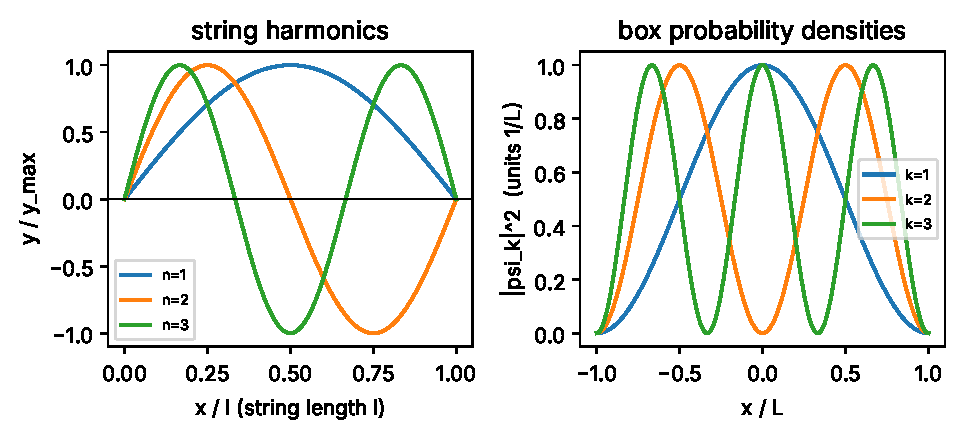
\includegraphics[width=0.85\linewidth]{figs/schrodinger_standing.pdf}
\caption{Left: the first three standing-wave shapes $\sin(n\pi x/\ell)$ of a string pinned at $x=0$ and $x=\ell$. Right: the first three probability densities $\abs{\psi_k}^2$ of a quantum particle in a box with impenetrable walls at $x=\pm L$ (derived in Sec.~\ref{sec:schrodinger-operators} and Sec.~\ref{sec:schrodinger-born}). The shapes are the same family of sines; the quantum picture plots the squared modulus, for reasons explained by the Born rule.}
\label{fig:schrodinger-standing}
\end{figure}

\begin{keyideas}
\item A sinusoid $\sin(kx-\omega t)$ solves the string wave equation only if $\omega=vk$; a relation $\omega(k)$ forced by a wave equation is its dispersion relation.
\item Boundary conditions (pinned ends) select a discrete set of allowed wavenumbers and frequencies: a spectrum.
\item Complex exponentials $e^{i(kx-\omega t)}$ package sines and cosines together; for strings the physics is in the real part.
\end{keyideas}

%======================================================================
\section{Matter waves: the de Broglie relation}\label{sec:schrodinger-debroglie}
%======================================================================

\subsection{Photons first}

We need two experimental facts from the early twentieth century. We take them on trust; HRW \cite{hrw} describes the experiments in its chapters on photons and matter waves. First, Planck (1900) and Einstein (1905) concluded that light of frequency $f$ exchanges energy with matter only in packets, called photons, of energy $E=hf$. Einstein was explaining the photoelectric effect, in which light knocks electrons out of a metal. Here $h=6.62607015\times10^{-34}$~J\,s is Planck's constant. Second, Compton's 1923 experiments, scattering X-rays from electrons, showed that each photon also carries momentum $p=h/\lambda$, with $\lambda$ the wavelength of the light. It is convenient to define the \emph{reduced Planck constant}
\begin{equation}
\hbar=\frac{h}{2\pi}=1.054571817\times10^{-34}\ \text{J\,s}
\end{equation}
(read ``h-bar''). Using $\omega=2\pi f$ and $k=2\pi/\lambda$,
\begin{equation}
E=hf=\frac{h}{2\pi}\,2\pi f=\hbar\omega,\qquad
p=\frac{h}{\lambda}=\frac{h}{2\pi}\cdot\frac{2\pi}{\lambda}=\hbar k.
\label{eq:schrodinger-planck}
\end{equation}
Energy is tied to angular frequency, momentum to angular wavenumber, and the exchange rate is $\hbar$ in both cases.

\subsection{De Broglie's hypothesis}

In 1924 Louis de Broglie proposed that the same relations hold for particles with mass: a particle of momentum $p$ has an associated wave of wavelength
\begin{equation}
\lambda=\frac{h}{p},\qquad\text{equivalently}\qquad p=\hbar k,\quad E=\hbar\omega.
\label{eq:schrodinger-debroglie}
\end{equation}
This was a hypothesis, not a deduction. It was confirmed in 1927 when Davisson and Germer, and independently G.~P.~Thomson, observed electrons diffracting from crystals exactly as waves of wavelength $h/p$ would. Diffraction is an interference effect, and interference is the signature of superposition: amplitudes add, and the intensity is computed from the sum.

\begin{sample}{De Broglie wavelengths of an electron and a baseball}
\textbf{Problem.} (a) Find the de Broglie wavelength of an electron with kinetic energy $K=100$~eV. (b) Find that of a baseball of mass $0.145$~kg moving at $40$~m/s. Use $m_e=9.1093837\times10^{-31}$~kg and $1~\text{eV}=1.602176634\times10^{-19}$~J.

\textbf{Step 1: momentum of the electron.} At $100$~eV the electron is far from relativistic (its rest energy is about half a million eV), so $K=p^2/2m_e$ and $p=\sqrt{2m_eK}$. In SI units $K=100\times1.602176634\times10^{-19}~\text{J}=1.602\times10^{-17}$~J, so
\[
p=\sqrt{2(9.109\times10^{-31})(1.602\times10^{-17})}~\text{kg\,m/s}=5.403\times10^{-24}~\text{kg\,m/s}.
\]

\textbf{Step 2: wavelength of the electron.}
\[
\lambda=\frac{h}{p}=\frac{6.626\times10^{-34}}{5.403\times10^{-24}}~\text{m}=1.226\times10^{-10}~\text{m}.
\]
This is comparable to the spacing of atoms in a crystal (a few tenths of a nanometer), which is why crystals diffract electrons.

\textbf{Step 3: the baseball.} $p=mv=(0.145)(40)=5.8$~kg\,m/s, so
\[
\lambda=\frac{6.626\times10^{-34}}{5.8}~\text{m}=1.14\times10^{-34}~\text{m},
\]
some twenty orders of magnitude smaller than an atomic nucleus. No slit or crystal can diffract it, which is why you never see a baseball interfere with itself.

\textbf{Answer.}
\[
\boxed{\lambda_e=0.1226~\text{nm},\qquad \lambda_{\rm ball}=1.14\times10^{-34}~\text{m}}
\]
\end{sample}

\begin{checkpoint}
A (nonrelativistic) electron's speed is doubled. By what factor does its de Broglie wavelength change? By what factor does its kinetic energy change?
\end{checkpoint}
\checkanswer{$p=mv$ doubles, so $\lambda=h/p$ halves. The kinetic energy $\tfrac12mv^2$ grows by a factor $4$. Equivalently $\lambda\propto1/\sqrt{K}$.}

\begin{pitfall}
Two common slips. (1) Using $h$ where $\hbar$ is meant, or the reverse: $\lambda=h/p$ but $k=p/\hbar$. They differ by $2\pi$. (2) Using the total energy, or $p=E/c$ (which is for light), for a massive slow particle. For a slow particle use $p=\sqrt{2mK}$ with $K$ the kinetic energy.
\end{pitfall}

\subsection{The free-particle dispersion relation}

For a free particle (no forces) the energy is all kinetic, $E=p^2/2m$. Substituting $E=\hbar\omega$ and $p=\hbar k$ from Eq.~\eqref{eq:schrodinger-debroglie},
\begin{equation}
\hbar\omega=\frac{(\hbar k)^2}{2m}
\quad\Longrightarrow\quad
\omega=\frac{\hbar k^2}{2m}.
\label{eq:schrodinger-free-dispersion}
\end{equation}
Compare with the string's $\omega=vk$ in Eq.~\eqref{eq:schrodinger-dispersion-string}: here $\omega$ grows as the \emph{square} of $k$. Matter waves are \emph{dispersive}: their phase velocity $\omega/k=\hbar k/2m$ depends on the wavelength. The right panel of \cref{fig:schrodinger-planewave}, which appears in Sec.~\ref{sec:schrodinger-tdse} and uses the units of Sec.~\ref{sec:schrodinger-units}, contrasts the two.

\begin{keyideas}
\item De Broglie: a particle of momentum $p$ carries a wave with $\lambda=h/p$; equivalently $p=\hbar k$ and $E=\hbar\omega$, with $\hbar=h/2\pi$.
\item The wavelength is observable (electron diffraction) only when it is comparable to some length in the experiment.
\item For a free particle $E=p^2/2m$ turns into the dispersion relation $\omega=\hbar k^2/2m$, quadratic rather than linear in $k$.
\end{keyideas}

%======================================================================
\section{Building a wave equation}\label{sec:schrodinger-tdse}
%======================================================================

If particles are waves, there should be a wave equation that tells the wave how to evolve, just as Eq.~\eqref{eq:schrodinger-wave} tells a string. Can we derive it? Honestly, no. We can only list requirements, guess the simplest equation that meets them, and then test the guess against experiment. That is what Erwin Schr\"odinger did in 1926, and it is what we do now.

\begin{beyond}
\textbf{Taken on trust: the Schr\"odinger equation itself.} The equation we arrive at below is a \emph{postulate} of quantum mechanics. Our argument shows that it is the simplest linear equation consistent with the de Broglie relations and $E=p^2/2m+V$; it does not prove that nature obeys it. Its justification is the agreement of its predictions (atomic spectra, chemistry, semiconductors, and much more) with experiment. Some deeper frameworks (for instance, deriving it from symmetry principles or from relativistic quantum field theory in a low-speed limit) exist but are beyond this book; see Griffiths and Schroeter \cite{griffiths} for the standard presentation and its experimental basis.
\end{beyond}

\subsection{The requirements}

We want an equation for a wave function $\Psi(x,t)$ (capital psi) such that:
\begin{enumerate}
\item[(R1)] It is \emph{linear}: if $\Psi_1$ and $\Psi_2$ are solutions, so is $a\Psi_1+b\Psi_2$ for any constants $a,b$. Electron diffraction shows interference, and interference requires that amplitudes superpose.
\item[(R2)] For a free particle, plane waves of wavenumber $k$ and angular frequency $\omega$ are solutions exactly when $\omega$ and $k$ obey Eq.~\eqref{eq:schrodinger-free-dispersion}.
\item[(R3)] The equation's coefficients do not depend on $k$ or $\omega$: one equation must serve every wavelength, so that superpositions of different $k$ also solve it.
\end{enumerate}

\subsection{The string equation fails}

Try Eq.~\eqref{eq:schrodinger-wave}. We showed it forces $\omega=vk$, linear in $k$. No constant $v$ can make $vk$ equal $\hbar k^2/2m$ for all $k$ (the ratio $\hbar k^2/2m\div k=\hbar k/2m$ changes with $k$). So the string equation cannot satisfy (R2) with a single constant $v$, and (R3) forbids letting $v$ depend on $k$.

\subsection{Counting derivatives}

Each time derivative of a plane wave brings down one factor of $\omega$; each space derivative brings down one factor of $k$. The dispersion relation \eqref{eq:schrodinger-free-dispersion} has $\omega$ to the first power and $k$ to the second. So we should try an equation with \emph{one} time derivative and \emph{two} space derivatives:
\begin{equation}
\frac{\partial\Psi}{\partial t}=\alpha\,\frac{\partial^2\Psi}{\partial x^2},
\label{eq:schrodinger-trial}
\end{equation}
with $\alpha$ a constant to be found.

\subsection{Real sinusoids cannot work}

Try a real wave, $\Psi=\cos(kx-\omega t)$. The left side of Eq.~\eqref{eq:schrodinger-trial} is
\[
\frac{\partial\Psi}{\partial t}=\omega\sin(kx-\omega t),
\]
and the right side is
\[
\alpha\frac{\partial^2\Psi}{\partial x^2}=-\alpha k^2\cos(kx-\omega t).
\]
A sine cannot equal a multiple of a cosine for all $x$ and $t$ (at a point where the cosine is zero and the sine is not, the right side vanishes and the left side does not), unless both coefficients vanish: $\omega=0$ and $\alpha k^2=0$. That is no wave at all. The same happens for $\sin(kx-\omega t)$. (Problem~4 at the end of this chapter redoes the cosine case in full, directly against the free Schr\"odinger equation.) One time derivative turns a cosine into a sine, while two space derivatives turn a cosine back into a cosine, and nothing real can reconcile them.

\subsection{Complex exponentials do work}

Now try the complex plane wave
\begin{equation}
\Psi(x,t)=e^{i(kx-\omega t)}=\cos(kx-\omega t)+i\sin(kx-\omega t).
\label{eq:schrodinger-planewave}
\end{equation}
We need the derivatives of $e^{i\theta}$. Using Euler's formula and differentiating the real and imaginary parts separately,
\[
\frac{\dd}{\dd\theta}e^{i\theta}=-\sin\theta+i\cos\theta=i(\cos\theta+i\sin\theta)=ie^{i\theta},
\]
where in the middle step we used $i\cdot i\sin\theta=-\sin\theta$. With the chain rule, $\theta=kx-\omega t$ gives $\partial\theta/\partial x=k$ and $\partial\theta/\partial t=-\omega$, so
\begin{align}
\frac{\partial\Psi}{\partial t}&=-i\omega\,\Psi,\label{eq:schrodinger-dt-plane}\\
\frac{\partial\Psi}{\partial x}&=ik\,\Psi,\\
\frac{\partial^2\Psi}{\partial x^2}&=(ik)(ik)\Psi=-k^2\Psi.\label{eq:schrodinger-dxx-plane}
\end{align}
Unlike the real case, both sides of Eq.~\eqref{eq:schrodinger-trial} are now multiples of the \emph{same} function $\Psi$. Substituting,
\[
-i\omega\Psi=-\alpha k^2\Psi
\quad\Longrightarrow\quad
\omega=\frac{\alpha k^2}{i}=-i\alpha k^2.
\]
We want $\omega=\hbar k^2/2m$, so we need $-i\alpha=\hbar/2m$, that is $\alpha=i\hbar/2m$ (check: $-i\cdot i\hbar/2m=\hbar/2m$, because $-i\cdot i=-i^2=1$). With this $\alpha$, Eq.~\eqref{eq:schrodinger-trial} becomes $\partial\Psi/\partial t=(i\hbar/2m)\partial^2\Psi/\partial x^2$. Multiply both sides by $i\hbar$ and use $i\hbar\cdot i\hbar/2m=-\hbar^2/2m$:
\begin{equation}
i\hbar\frac{\partial\Psi}{\partial t}=-\frac{\hbar^2}{2m}\frac{\partial^2\Psi}{\partial x^2}.
\label{eq:schrodinger-free}
\end{equation}
This is the free Schr\"odinger equation. The factor $i$ is essential, and with it the wave function is necessarily complex.

There is a nice way to read Eq.~\eqref{eq:schrodinger-free}. On a plane wave, Eq.~\eqref{eq:schrodinger-dt-plane} says $i\hbar\,\partial\Psi/\partial t=\hbar\omega\Psi=E\Psi$, and Eq.~\eqref{eq:schrodinger-dxx-plane} says $-(\hbar^2/2m)\partial^2\Psi/\partial x^2=(\hbar^2k^2/2m)\Psi=(p^2/2m)\Psi$. So the equation is the energy statement $E=p^2/2m$, with the replacements
\begin{equation}
E\ \longrightarrow\ i\hbar\frac{\partial}{\partial t},\qquad p\ \longrightarrow\ -i\hbar\frac{\partial}{\partial x}.
\label{eq:schrodinger-replacements}
\end{equation}
(Check the second: $-i\hbar\,\partial\Psi/\partial x=-i\hbar\cdot ik\Psi=\hbar k\Psi=p\Psi$.) From here on we sometimes abbreviate $\partial/\partial t$ as $\partial_t$, $\partial/\partial x$ as $\partial_x$ and $\partial^2/\partial x^2$ as $\partial_x^2$, and similarly for other variables. We also write $y_{xx}$ for $\partial^2y/\partial x^2$, $y_{tt}$ for $\partial^2y/\partial t^2$ and $\Psi_t$ for $\partial\Psi/\partial t$.

\subsection{Adding a potential}

A particle moving in a potential energy $V(x)$ has $E=p^2/2m+V(x)$. Applying the same replacements, and letting $V(x)$ simply multiply $\Psi$, gives the \emph{time-dependent Schr\"odinger equation}
\begin{equation}
\boxed{\;i\hbar\frac{\partial\Psi}{\partial t}=-\frac{\hbar^2}{2m}\frac{\partial^2\Psi}{\partial x^2}+V(x)\,\Psi\;}
\label{eq:schrodinger-tdse}
\end{equation}
For a free particle this is the simplest equation meeting (R1)--(R3), given the convention $e^{i(kx-\omega t)}$ for a right-moving wave; it is still a guess. With $V\neq0$ we have \emph{guessed} further, by analogy; this is the step that experiment, not logic, must validate.

\paragraph{Linearity.} Suppose $\Psi_1$ and $\Psi_2$ both solve Eq.~\eqref{eq:schrodinger-tdse} and $\Psi=a\Psi_1+b\Psi_2$ with constants $a,b$. Derivatives are linear, so
\begin{align*}
i\hbar\frac{\partial\Psi}{\partial t}
&=a\,i\hbar\frac{\partial\Psi_1}{\partial t}+b\,i\hbar\frac{\partial\Psi_2}{\partial t}\\
&=a\left(-\frac{\hbar^2}{2m}\Psi_1''+V\Psi_1\right)+b\left(-\frac{\hbar^2}{2m}\Psi_2''+V\Psi_2\right)\quad\text{(each solves the equation)}\\
&=-\frac{\hbar^2}{2m}\left(a\Psi_1+b\Psi_2\right)''+V\left(a\Psi_1+b\Psi_2\right)\quad\text{(collect terms)},
\end{align*}
where a prime means $\partial/\partial x$. So $\Psi$ solves it too: requirement (R1) holds.

\begin{figure}[htbp]\centering
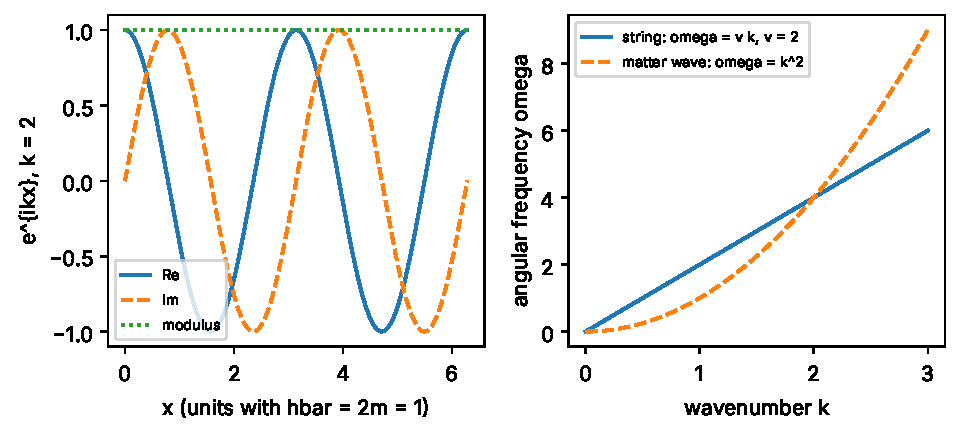
\includegraphics[width=0.85\linewidth]{figs/schrodinger_planewave.pdf}
\caption{Left: real part (solid) and imaginary part (dashed) of the plane wave $e^{ikx}$ at $t=0$, with $k=2$ (in units $\hbar=2m=1$ of Sec.~\ref{sec:schrodinger-units}); the modulus $\abs{e^{ikx}}=1$ (dotted) is constant. Right: dispersion relations. A string has $\omega=vk$ (here $v=2$); a free matter wave has $\omega=\hbar k^2/2m$, which is $\omega=k^2$ in units $\hbar=2m=1$.}
\label{fig:schrodinger-planewave}
\end{figure}

\begin{checkpoint}
Why can a guitar string get away with a real displacement $y(x,t)$, while the matter wave $\Psi$ must be complex?
\end{checkpoint}
\checkanswer{The string equation has two time derivatives, which turn a cosine back into a cosine, matching the two space derivatives. The Schr\"odinger equation has one time derivative (forced by $\omega\propto k^2$), which turns a cosine into a sine; only the complex combination $e^{i\theta}$, whose derivative is a multiple of itself, can satisfy it.}

\subsection{Phase velocity, group velocity and the particle's speed}

Here is a puzzle that tests the equation. A free electron with momentum $p$ moves at $v=p/m$. What does the wave do?

\begin{sample}{A free electron wave}
\textbf{Problem.} An electron is described by a plane wave with $k=1.0\times10^{10}~\text{m}^{-1}$. Find (a) its kinetic energy in eV, (b) $\omega$, (c) the phase velocity, and (d) the classical speed $p/m$. Use $\hbar=1.054571817\times10^{-34}$~J\,s and $m_e=9.1093837\times10^{-31}$~kg.

\textbf{Step 1: energy.} $K=p^2/2m=\hbar^2k^2/2m$:
\[
K=\frac{(1.0546\times10^{-34})^2(1.0\times10^{20})}{2(9.109\times10^{-31})}~\text{J}=6.104\times10^{-19}~\text{J}=3.81~\text{eV}.
\]

\textbf{Step 2: angular frequency.} $\omega=K/\hbar=\hbar k^2/2m$:
\[
\omega=\frac{6.104\times10^{-19}}{1.0546\times10^{-34}}~\text{rad/s}=5.79\times10^{15}~\text{rad/s}.
\]

\textbf{Step 3: phase velocity.} $v_{\rm ph}=\omega/k=5.79\times10^{15}/10^{10}~\text{m/s}=5.79\times10^{5}$~m/s.

\textbf{Step 4: classical speed.} $p/m=\hbar k/m=(1.0546\times10^{-24})/(9.109\times10^{-31})~\text{m/s}=1.16\times10^6$~m/s.

\textbf{Answer.}
\[
\boxed{K=3.81~\text{eV},\ \ \omega=5.79\times10^{15}~\text{rad/s},\ \ v_{\rm ph}=5.79\times10^5~\text{m/s},\ \ p/m=1.16\times10^6~\text{m/s}}
\]
The crests move at exactly \emph{half} the particle's speed: $v_{\rm ph}=\hbar k/2m$ while $p/m=\hbar k/m$.
\end{sample}

The resolution of the factor of two uses beats (Chapter~\ref{ch:fourier-series}). A real particle is not an infinite plane wave but a localized bump, a superposition of nearby wavenumbers. Take two complex plane waves $e^{i(k_1x-\omega_1t)}$ and $e^{i(k_2x-\omega_2t)}$, with $k_1=k-\tfrac12\Delta k$ and $k_2=k+\tfrac12\Delta k$. Their frequencies $\omega_1,\omega_2$ are given by the dispersion relation, and we write $\Delta\omega=\omega_2-\omega_1$. By linearity their sum solves the free Schr\"odinger equation. Look at the real part of the sum, $\cos A+\cos B$; the imaginary part, $\sin A+\sin B$, behaves the same way. The identity $\cos A+\cos B=2\cos\frac{A-B}{2}\cos\frac{A+B}{2}$ with $A=k_2x-\omega_2t$, $B=k_1x-\omega_1t$ gives
\[
\cos A+\cos B=2\cos\!\left(\frac{\Delta k\,x-\Delta\omega\,t}{2}\right)\cos\!\left(\frac{(k_1+k_2)x-(\omega_1+\omega_2)t}{2}\right).
\]
The first factor is a slowly varying \emph{envelope}; its shape is unchanged when $\Delta k\,x-\Delta\omega\,t$ is constant, so the envelope moves at $\Delta\omega/\Delta k$. As $\Delta k\to0$ this becomes the \emph{group velocity}
\begin{equation}
v_{\rm g}=\frac{\dd\omega}{\dd k}=\frac{\dd}{\dd k}\frac{\hbar k^2}{2m}=\frac{\hbar k}{m}=\frac{p}{m}.
\label{eq:schrodinger-group}
\end{equation}
The bump, which is where the particle is likely to be found, travels at exactly the classical speed. The Schr\"odinger equation passes its first test.

\begin{pitfall}
The phase velocity of a matter wave is not the particle's speed; the group velocity is. For the string the two coincide because $\omega=vk$ is linear, which is why first-year physics never needed to distinguish them.
\end{pitfall}

\begin{keyideas}
\item The simplest linear equation whose plane-wave solutions obey $\hbar\omega=\hbar^2k^2/2m$ has one time derivative and two space derivatives, and it requires the factor $i$: Eq.~\eqref{eq:schrodinger-free}.
\item With a potential, $E=p^2/2m+V$ and the replacements $E\to i\hbar\,\partial_t$, $p\to-i\hbar\,\partial_x$ give the time-dependent Schr\"odinger equation \eqref{eq:schrodinger-tdse}, a postulate checked by experiment.
\item The equation is linear, so solutions superpose. Wave packets move at the group velocity $\dd\omega/\dd k=p/m$, the classical speed.
\end{keyideas}

%======================================================================
\section{Separation of variables and stationary states}\label{sec:schrodinger-separation}
%======================================================================

Equation~\eqref{eq:schrodinger-tdse} involves both $x$ and $t$. When $V$ depends on $x$ only (as it always will in this book), a standard trick splits it into two simpler equations.

\subsection{The separation}

Look for solutions that are a product of a function of $x$ and a function of $t$:
\begin{equation}
\Psi(x,t)=\psi(x)\,\varphi(t).
\label{eq:schrodinger-sep}
\end{equation}
Then $\partial\Psi/\partial t=\psi\,\dd\varphi/\dd t$ and $\partial^2\Psi/\partial x^2=\varphi\,\dd^2\psi/\dd x^2$. Substituting into Eq.~\eqref{eq:schrodinger-tdse},
\[
i\hbar\,\psi\frac{\dd\varphi}{\dd t}=-\frac{\hbar^2}{2m}\varphi\frac{\dd^2\psi}{\dd x^2}+V\psi\varphi.
\]
Divide both sides by $\psi\varphi$ (at points where it is not zero):
\begin{equation}
i\hbar\,\frac{1}{\varphi}\frac{\dd\varphi}{\dd t}
=\frac{1}{\psi}\left(-\frac{\hbar^2}{2m}\frac{\dd^2\psi}{\dd x^2}+V\psi\right).
\end{equation}
The left side depends only on $t$; the right side depends only on $x$. Fix $x$ and vary $t$: the right side does not change, so the left side cannot change either. Fix $t$ and vary $x$: by the same argument the right side is constant. So both sides equal a single constant, which we call $E$ (we will see in a moment that it is the energy). That gives two ordinary differential equations:
\begin{align}
i\hbar\frac{\dd\varphi}{\dd t}&=E\,\varphi,\label{eq:schrodinger-time-ode}\\
-\frac{\hbar^2}{2m}\frac{\dd^2\psi}{\dd x^2}+V(x)\psi&=E\,\psi.\label{eq:schrodinger-tise}
\end{align}

\subsection{The time factor}

Equation~\eqref{eq:schrodinger-time-ode} says $\dd\varphi/\dd t=(E/i\hbar)\varphi=-i(E/\hbar)\varphi$, using $1/i=-i$. We claim the solution is
\begin{equation}
\varphi(t)=e^{-iEt/\hbar}.
\label{eq:schrodinger-timefactor}
\end{equation}
Check, with $\omega=E/\hbar$: $e^{-i\omega t}=\cos\omega t-i\sin\omega t$, so
\[
\frac{\dd}{\dd t}e^{-i\omega t}=-\omega\sin\omega t-i\omega\cos\omega t=-i\omega(\cos\omega t-i\sin\omega t)=-i\omega e^{-i\omega t},
\]
where we used $-i\omega\cdot(-i\sin\omega t)=i^2\omega\sin\omega t=-\omega\sin\omega t$. So $\varphi'=-i(E/\hbar)\varphi$ as required. (Any constant multiple of $\varphi$ also works; we absorb that constant into $\psi$. There are no other solutions. If $\varphi$ solves the equation, then by the product rule $\frac{\dd}{\dd t}\left(\varphi e^{iEt/\hbar}\right)=\varphi'e^{iEt/\hbar}+\frac{iE}{\hbar}\varphi e^{iEt/\hbar}=\left(-\frac{iE}{\hbar}+\frac{iE}{\hbar}\right)\varphi e^{iEt/\hbar}=0$. So $\varphi e^{iEt/\hbar}$ is a constant, and $\varphi$ is that constant times $e^{-iEt/\hbar}$.) The time factor rotates in the complex plane at angular frequency $\omega=E/\hbar$, exactly the de Broglie relation $E=\hbar\omega$, which justifies calling $E$ the energy.

\subsection{Why such states are called stationary}

For the separated solution $\Psi=\psi(x)e^{-iEt/\hbar}$, with $E$ real (we prove $E$ is real in Sec.~\ref{sec:schrodinger-hermitian}),
\begin{equation}
\abs{\Psi(x,t)}^2=\Psi^*\Psi=\psi^*(x)e^{+iEt/\hbar}\,\psi(x)e^{-iEt/\hbar}=\abs{\psi(x)}^2.
\end{equation}
The squared modulus does not depend on time. In Sec.~\ref{sec:schrodinger-born} we will see that $\abs{\Psi}^2$ is what is measured, so nothing observable about such a state changes in time. These solutions are called \emph{stationary states}; each one is a standing wave whose overall phase turns like the hand of a clock.

\subsection{The time-independent Schr\"odinger equation}

Equation~\eqref{eq:schrodinger-tise} is the \emph{time-independent Schr\"odinger equation}. It contains no time at all: it asks for functions $\psi(x)$ and numbers $E$ such that a certain combination of $\psi$ and its second derivative is a multiple $E$ of $\psi$ itself. That is an eigenvalue problem, the subject of Sec.~\ref{sec:schrodinger-operators}.

\begin{sample}{How fast does the phase of a stationary state turn?}
\textbf{Problem.} A stationary state has $E=1.00$~eV. How long does the phase factor $e^{-iEt/\hbar}$ take to make one full turn around the unit circle?

\textbf{Step 1:} One full turn means $Et/\hbar=2\pi$, so the period is $T_{\rm ph}=2\pi\hbar/E=h/E$.

\textbf{Step 2:} With $E=1.602176634\times10^{-19}$~J,
\[
T_{\rm ph}=\frac{6.62607\times10^{-34}}{1.602177\times10^{-19}}~\text{s}=4.14\times10^{-15}~\text{s}.
\]

\textbf{Answer.} \[\boxed{T_{\rm ph}=4.14\times10^{-15}~\text{s}}\]
A few femtoseconds. But since $\abs{\Psi}^2$ is unchanged, no experiment on this single state can see the rotation; only \emph{differences} of energies between superposed states produce observable time dependence (Sec.~\ref{sec:schrodinger-expectation}).
\end{sample}

\subsection{General solutions from stationary states}

Suppose we have found many solutions $(\psi_n,E_n)$, $n=1,2,\dots$, of Eq.~\eqref{eq:schrodinger-tise}. Each product $\psi_n(x)e^{-iE_nt/\hbar}$ solves Eq.~\eqref{eq:schrodinger-tdse} (that is how we built them), and by linearity so does any sum
\begin{equation}
\Psi(x,t)=\sum_n c_n\,\psi_n(x)\,e^{-iE_nt/\hbar},
\label{eq:schrodinger-general}
\end{equation}
with constants $c_n$. At $t=0$ this is $\sum_nc_n\psi_n(x)$. If the $\psi_n$ can build any initial wave function (the expansion question of Sec.~\ref{sec:schrodinger-expectation}, similar to a Fourier series in Chapter~\ref{ch:fourier-series}), then Eq.~\eqref{eq:schrodinger-general} solves the whole time-dependent problem: find the stationary states once, then attach the clock factors. Given completeness of the stationary states (taken on trust in the \texttt{beyond} box of Sec.~\ref{sec:schrodinger-hermitian}), the whole time evolution of the system is encoded in the stationary states and their energies. The paper goes further and never considers time evolution at all: it uses only the eigenvalues $E_n$ and eigenfunctions $\psi_n$ of $H$.

\begin{checkpoint}
Is a superposition $\Psi=\psi_1e^{-iE_1t/\hbar}+\psi_2e^{-iE_2t/\hbar}$ with $E_1\neq E_2$ a stationary state?
\end{checkpoint}
\checkanswer{No. It solves the Schr\"odinger equation, but it is not of the form $\psi(x)\varphi(t)$, and its $\abs{\Psi}^2$ contains a cross term oscillating at $(E_2-E_1)/\hbar$ (computed in Sec.~\ref{sec:schrodinger-expectation}), so observable properties change in time.}

\begin{keyideas}
\item For $V=V(x)$, the product $\psi(x)e^{-iEt/\hbar}$ solves the Schr\"odinger equation whenever $\psi$ and $E$ solve the time-independent equation \eqref{eq:schrodinger-tise}.
\item Such stationary states have time-independent $\abs{\Psi}^2$; their phase rotates at $\omega=E/\hbar$.
\item Superpositions of stationary states with clock factors attached give the general time evolution, Eq.~\eqref{eq:schrodinger-general}.
\end{keyideas}

%======================================================================
\section{The Hamiltonian as an operator}\label{sec:schrodinger-operators}
%======================================================================

\subsection{Operators}

An \emph{operator} is a rule that takes a function and returns another function. We write operators with hats or capital letters. Three examples:
\begin{itemize}
\item the derivative operator $D$: $Df=\dd f/\dd x$;
\item a multiplication operator: $(\hat V f)(x)=V(x)f(x)$, ``multiply by the function $V$'';
\item the second-derivative operator $D^2f=\dd^2 f/\dd x^2$.
\end{itemize}
An operator $Q$ is \emph{linear} if $Q(af+bg)=aQf+bQg$ for all functions $f,g$ and constants $a,b$. All three examples are linear (derivatives of sums are sums of derivatives, and $V(af+bg)=aVf+bVg$). Linear operators on functions are the continuous cousins of matrices acting on vectors (Chapter~\ref{ch:linear-algebra}); in Sec.~\ref{sec:schrodinger-hermitian} we will make the analogy concrete by sampling functions on a grid.

\subsection{The Hamiltonian}

Define the \emph{Hamiltonian operator}
\begin{equation}
H=-\frac{\hbar^2}{2m}\frac{\dd^2}{\dd x^2}+V(x),
\qquad
H\psi=-\frac{\hbar^2}{2m}\psi''+V\psi.
\label{eq:schrodinger-H}
\end{equation}
It is named after W.~R.~Hamilton, whose classical ``Hamiltonian'' is the energy written as a function of position and momentum, $p^2/2m+V(x)$; the replacement $p\to-i\hbar\,\dd/\dd x$ of Eq.~\eqref{eq:schrodinger-replacements} turns $p^2$ into $(-i\hbar)^2\dd^2/\dd x^2=-\hbar^2\dd^2/\dd x^2$, which is how the first term arises. With this notation the time-independent equation \eqref{eq:schrodinger-tise} is simply
\begin{equation}
\boxed{\;H\psi=E\psi\;}
\label{eq:schrodinger-eigen}
\end{equation}
and the time-dependent equation \eqref{eq:schrodinger-tdse} is $i\hbar\,\partial\Psi/\partial t=H\Psi$.

Compare with a matrix eigenvalue problem $\mathbf{A}\mathbf{v}=\lambda\mathbf{v}$ (Chapter~\ref{ch:eigen}). The operator $H$ plays the role of $\mathbf{A}$, the function $\psi$ the role of the eigenvector $\mathbf{v}$, and $E$ the role of $\lambda$. The solutions $\psi$ are called \emph{eigenfunctions} of $H$ and the numbers $E$ its \emph{eigenvalues}, or \emph{energy levels}. A pair $(E_n,\psi_n)$ is an \emph{eigenpair}.

\subsection{Boundary conditions belong to the operator}

As with the string, the allowed $E$ depend on boundary conditions. In this book (and in the paper) the particle lives in a box $[-L,L]$ with impenetrable walls, which means $V=+\infty$ outside the box and the wave function must vanish at the walls:
\begin{equation}
\psi(-L)=\psi(L)=0.
\label{eq:schrodinger-dirichlet}
\end{equation}
Conditions that fix the value of the function at the boundary are called \emph{Dirichlet} conditions. When we speak of ``the operator $H$ on $[-L,L]$ with Dirichlet walls'' we mean the formula \eqref{eq:schrodinger-H} \emph{together with} the rule that it acts only on functions obeying Eq.~\eqref{eq:schrodinger-dirichlet}. Changing the boundary conditions changes the operator, and therefore its eigenvalues. (Why $\psi$ must vanish at an infinite wall is argued physically in Chapter~\ref{ch:bound-states}; here we take it as the definition of the box.)

\begin{sample}{Eigenfunctions of the empty box}
\textbf{Problem.} Take $V=0$ inside $[-L,L]$ with Dirichlet walls. Show that for every positive integer $k$ the function
\[
\psi_k(x)=\sin\!\left(\frac{k\pi(x+L)}{2L}\right)
\]
is an eigenfunction of $H$, and find its eigenvalue.

\textbf{Step 1: boundary conditions.} At $x=-L$ the argument is $0$ and $\sin0=0$. At $x=L$ the argument is $k\pi\cdot2L/2L=k\pi$, and $\sin(k\pi)=0$ for integer $k$. Both walls are satisfied.

\textbf{Step 2: first derivative.} Write $q=k\pi/2L$, so $\psi_k=\sin(q(x+L))$. By the chain rule $\psi_k'=q\cos(q(x+L))$.

\textbf{Step 3: second derivative.} $\psi_k''=-q^2\sin(q(x+L))=-q^2\psi_k$.

\textbf{Step 4: apply $H$.} With $V=0$, $H\psi_k=-\frac{\hbar^2}{2m}\psi_k''=\frac{\hbar^2}{2m}q^2\psi_k$.

\textbf{Answer.}
\[
\boxed{E_k=\frac{\hbar^2}{2m}\left(\frac{k\pi}{2L}\right)^2,\qquad k=1,2,3,\dots}
\]
This is the fixed-end string problem of Chapter~\ref{ch:eigen} again, with eigenvalue $(k\pi/2L)^2$ multiplied by $\hbar^2/2m$. Chapter~\ref{ch:bound-states} solves the box problem fully, including the question of whether there are any other eigenfunctions. Note $k=0$ gives $\psi=0$, which is not allowed (an eigenfunction must be nonzero), and negative $k$ gives $-\psi_{\abs{k}}$, the same state up to sign.
\end{sample}

We record the empty-box levels as a numbered equation:
\begin{equation}
E_k=\frac{\hbar^2}{2m}\left(\frac{k\pi}{2L}\right)^2,\qquad k=1,2,3,\dots
\label{eq:schrodinger-box-levels}
\end{equation}
The integer $k$ that labels the empty-box states should not be confused with the wavenumber $k$ of a plane wave; for the box state $\psi_k$ the wavenumber is $q=k\pi/2L$. The paper labels levels by $n$ and reserves $k$ for its cosine basis functions $\cos(k\pi x/L)$. In Sec.~\ref{sec:schrodinger-paper} we switch to $n$ for levels.

\subsection{The momentum operator}

Equation~\eqref{eq:schrodinger-replacements} suggests defining the \emph{momentum operator}
\begin{equation}
\hat p=-i\hbar\frac{\dd}{\dd x}.
\label{eq:schrodinger-momentum}
\end{equation}
The plane wave $e^{ikx}$ is an eigenfunction: $\hat p\,e^{ikx}=-i\hbar\cdot ik\,e^{ikx}=\hbar k\,e^{ikx}$, with eigenvalue $\hbar k=p$. Then $\hat p^2=\hat p\hat p=(-i\hbar)^2\dd^2/\dd x^2=-\hbar^2\dd^2/\dd x^2$ and
\begin{equation}
H=\frac{\hat p^2}{2m}+V(x),
\end{equation}
the operator version of ``kinetic plus potential energy''. A box state $\psi_k$ is \emph{not} an eigenfunction of $\hat p$: writing $\sin\theta=(e^{i\theta}-e^{-i\theta})/2i$ (Chapter~\ref{ch:complex}) shows it is a superposition of waves moving left and right, just like the standing wave \eqref{eq:schrodinger-standing}.

\begin{checkpoint}
Is the function $\psi(x)=\cos(\pi x/2L)$ an eigenfunction of the empty-box Hamiltonian on $[-L,L]$? If so, which $k$ does it correspond to?
\end{checkpoint}
\checkanswer{Yes. $\sin(\pi(x+L)/2L)=\sin(\pi x/2L+\pi/2)=\cos(\pi x/2L)$, so it is $\psi_1$, with $E_1=\frac{\hbar^2}{2m}(\pi/2L)^2$. It vanishes at $x=\pm L$ because $\cos(\pm\pi/2)=0$.}

\begin{keyideas}
\item An operator maps functions to functions; the Hamiltonian $H=-\frac{\hbar^2}{2m}\frac{\dd^2}{\dd x^2}+V(x)$ is the energy operator.
\item The time-independent Schr\"odinger equation is the eigenvalue problem $H\psi=E\psi$: eigenfunctions are stationary states, eigenvalues are energy levels.
\item Boundary conditions are part of the operator. In the empty box with Dirichlet walls, $E_k=\frac{\hbar^2}{2m}(k\pi/2L)^2$.
\item The momentum operator is $\hat p=-i\hbar\,\dd/\dd x$, and $H=\hat p^2/2m+V$.
\end{keyideas}

%======================================================================
\section{What the wavefunction means: the Born rule}\label{sec:schrodinger-born}
% DYK-BEGIN
\begin{didyouknow}{Physics in a Footnote}
Max Born's 1926 paper on collisions introduced the idea that the wavefunction gives \emph{probabilities}. The crucial point, that the probability is proportional to the \emph{square} of the wavefunction, appeared in a footnote added in proof. Born received the Nobel Prize in Physics for this statistical interpretation in 1954, nearly three decades later.
\end{didyouknow}
% DYK-END
%======================================================================

\subsection{The Born rule}

So far $\Psi$ is a complex wave with no stated meaning. The interpretation used by every working physicist was proposed by Max Born in 1926:

\begin{quote}
\textbf{Born rule.} If a particle has wave function $\Psi(x,t)$, the probability of finding it between $x$ and $x+\dd x$ when its position is measured at time $t$ is $\abs{\Psi(x,t)}^2\,\dd x$. The probability of finding it in an interval $[a,b]$ is
\begin{equation}
P_{[a,b]}(t)=\int_a^b\abs{\Psi(x,t)}^2\,\dd x.
\label{eq:schrodinger-born}
\end{equation}
\end{quote}

So $\abs{\Psi}^2$ is a \emph{probability density}: probability per unit length, with units of $1/\text{length}$ in one dimension. The wave function itself is called a \emph{probability amplitude}. Like the Schr\"odinger equation, the Born rule is a postulate.

\begin{beyond}
\textbf{Taken on trust: the Born rule and measurement.} Why squared moduli give probabilities, and what exactly happens during a measurement, are questions about the foundations of quantum mechanics that remain debated. Nothing in this book or in the paper depends on how they are answered; we need only the rule \eqref{eq:schrodinger-born} and its extension to energy measurements (Sec.~\ref{sec:schrodinger-expectation}). See Griffiths and Schroeter \cite{griffiths}, Chapter~1 and the Afterword, for a careful discussion.
\end{beyond}

Two consequences follow at once. Because the total probability of finding the particle \emph{somewhere} is one,
\begin{equation}
\int_{\text{all }x}\abs{\Psi(x,t)}^2\,\dd x=1.
\label{eq:schrodinger-norm}
\end{equation}
A wave function obeying this is \emph{normalized}. And because $\abs{e^{i\alpha}\Psi}^2=\abs{e^{i\alpha}}^2\abs{\Psi}^2=\abs{\Psi}^2$ for any real constant $\alpha$, multiplying a wave function by a constant phase $e^{i\alpha}$ changes no prediction: $\Psi$ and $e^{i\alpha}\Psi$ describe the same physical state. (This is why the overall sign of a single eigenvector returned by a numerical solver does not affect quantities such as $\abs{\psi_n}^2$. Relative signs between different states are another matter, as a checkpoint in Sec.~\ref{sec:schrodinger-expectation} shows.)

\subsection{Normalizing a wave function}

The Schr\"odinger equation is linear, so if $\psi$ is a solution then $A\psi$ is too, for any constant $A$. Normalization fixes $\abs{A}$: choose it so that Eq.~\eqref{eq:schrodinger-norm} holds.

\begin{sample}{Normalizing a cusp}
\textbf{Problem.} A wave function on the whole line is $\psi(x)=A\,e^{-\abs{x}/a}$ with $a>0$. (a) Find $A>0$ that normalizes it. (b) Find the probability that the particle is found within $\abs{x}<a$.

\textbf{Step 1: the normalization integral.} $\abs{\psi}^2=A^2e^{-2\abs{x}/a}$, an even function, so the integral over the line is twice the integral over $x>0$:
\[
\int_{-\infty}^{\infty}A^2e^{-2\abs{x}/a}\,\dd x=2A^2\int_0^\infty e^{-2x/a}\,\dd x.
\]

\textbf{Step 2: evaluate.} $\int_0^\infty e^{-2x/a}\dd x=\left[-\tfrac a2e^{-2x/a}\right]_0^\infty=0-\left(-\tfrac a2\right)=\tfrac a2$. So the integral is $2A^2\cdot a/2=A^2a$.

\textbf{Step 3: set it to 1.} $A^2a=1$, so $A=1/\sqrt a$.

\textbf{Step 4: probability within $\abs x<a$.} Again use evenness:
\[
P=2\cdot\frac1a\int_0^a e^{-2x/a}\dd x=\frac2a\left[-\frac a2e^{-2x/a}\right]_0^a=\frac2a\cdot\frac a2\left(1-e^{-2}\right)=1-e^{-2}.
\]

\textbf{Answer.}
\[
\boxed{A=\frac1{\sqrt a},\qquad P(\abs x<a)=1-e^{-2}=0.8647}
\]
The answer does not depend on $a$: $a$ only sets the scale. \Cref{fig:schrodinger-born} shows the density and the shaded probability.
\end{sample}

\begin{figure}[htbp]\centering
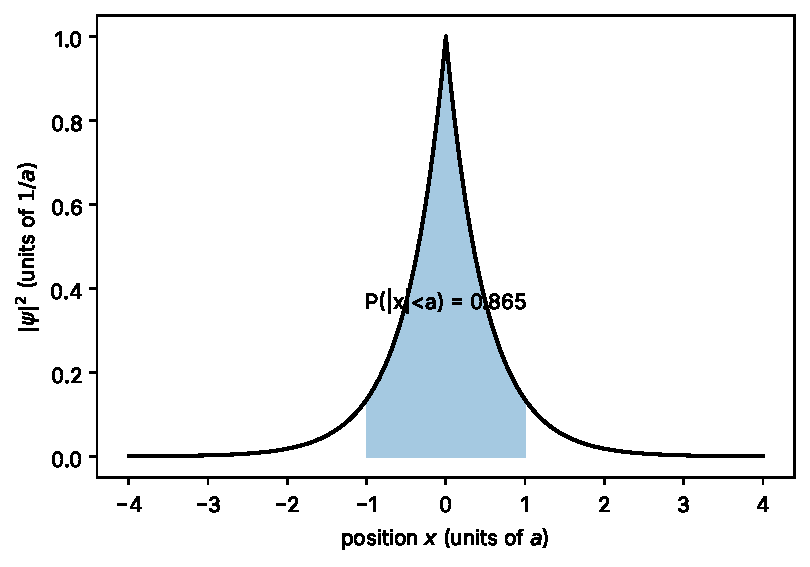
\includegraphics[width=0.85\linewidth]{figs/schrodinger_born.pdf}
\caption{The Born rule for the normalized wave function $\psi=a^{-1/2}e^{-\abs x/a}$ (here $a=1$, length in units of $a$). The curve is the probability density $\abs\psi^2=a^{-1}e^{-2\abs x/a}$ (units $1/a$); the total area under it is $1$, and the shaded area, the probability of finding the particle in $\abs x<a$, is $1-e^{-2}\approx0.865$.}
\label{fig:schrodinger-born}
\end{figure}

\begin{sample}{The box ground state}
\textbf{Problem.} The empty-box ground state on $[-L,L]$ is $\psi_1=A\sin(\pi(x+L)/2L)$. (a) Normalize it. (b) Find the probability that the particle is in the middle half, $-L/2<x<L/2$.

\textbf{Step 1: substitution.} Let $u=\pi(x+L)/2L$. Then $\dd x=(2L/\pi)\dd u$, and $x=-L,\,L$ map to $u=0,\,\pi$.

\textbf{Step 2: normalization integral.} Using $\sin^2u=\tfrac12(1-\cos2u)$,
\[
\int_{-L}^{L}A^2\sin^2\!\left(\frac{\pi(x+L)}{2L}\right)\dd x
=A^2\frac{2L}{\pi}\int_0^\pi\sin^2u\,\dd u
=A^2\frac{2L}{\pi}\left[\frac u2-\frac{\sin2u}{4}\right]_0^\pi
=A^2\frac{2L}{\pi}\cdot\frac\pi2=A^2L.
\]
So $A=1/\sqrt L$.

\textbf{Step 3: limits for the middle half.} $x=-L/2$ gives $u=\pi(L/2)/2L=\pi/4$; $x=L/2$ gives $u=\pi(3L/2)/2L=3\pi/4$.

\textbf{Step 4: integrate.}
\[
P=\frac1L\cdot\frac{2L}{\pi}\left[\frac u2-\frac{\sin2u}4\right]_{\pi/4}^{3\pi/4}
=\frac2\pi\left[\left(\frac{3\pi}8-\frac{\sin(3\pi/2)}4\right)-\left(\frac\pi8-\frac{\sin(\pi/2)}4\right)\right].
\]
With $\sin(3\pi/2)=-1$ and $\sin(\pi/2)=1$, the bracket is $\frac{3\pi}8+\frac14-\frac\pi8+\frac14=\frac\pi4+\frac12$.

\textbf{Answer.}
\[
\boxed{A=\frac1{\sqrt L},\qquad P=\frac2\pi\left(\frac\pi4+\frac12\right)=\frac12+\frac1\pi=0.8183}
\]
A classical particle bouncing at constant speed would spend exactly half its time in the middle half. The quantum ground state piles probability toward the center, where $\sin^2$ peaks (\cref{fig:schrodinger-standing}, right).
\end{sample}

The same calculation works for every box state. For $\psi_k=A\sin(k\pi(x+L)/2L)$ substitute $u=k\pi(x+L)/2L$, so that $\dd x=(2L/k\pi)\dd u$ and $u$ runs from $0$ to $k\pi$. Since
\[
\int_0^{k\pi}\sin^2u\,\dd u=\left[\frac u2-\frac{\sin2u}4\right]_0^{k\pi}=\frac{k\pi}2\quad\text{(because $\sin2k\pi=0$)},
\]
the normalization integral is $A^2\cdot\frac{2L}{k\pi}\cdot\frac{k\pi}{2}=A^2L$, and again $A=1/\sqrt L$. So the normalized empty-box states are
\begin{equation}
\psi_k(x)=\frac1{\sqrt L}\sin\!\left(\frac{k\pi(x+L)}{2L}\right),\qquad k=1,2,\dots
\label{eq:schrodinger-box-states}
\end{equation}

\begin{checkpoint}
Is $\psi(x)=2\sin(\pi(x+L)/2L)$ normalized on $[-L,L]$? If not, what is $\int\abs\psi^2\dd x$?
\end{checkpoint}
\checkanswer{No. Doubling $\psi$ multiplies $\abs\psi^2$ by 4, so the integral is $4L$ instead of $1$ (using Step 2 of the previous Sample Problem with $A=2$). It describes the same physical state as the normalized $\psi_1$ but must be rescaled before applying the Born rule.}

\subsection{Normalization is preserved in time}

There is a consistency question. Normalization is imposed at one time. If the Schr\"odinger equation let $\int\abs\Psi^2$ drift, total probability would stop being one. Let us prove it does not drift, and see exactly which property of $H$ is responsible.

Start from Eq.~\eqref{eq:schrodinger-tdse} and divide by $i\hbar$, using $1/i=-i$:
\begin{equation}
\frac{\partial\Psi}{\partial t}=\frac{i\hbar}{2m}\frac{\partial^2\Psi}{\partial x^2}-\frac{i}{\hbar}V\Psi.
\label{eq:schrodinger-dPsidt}
\end{equation}
(Check the first coefficient: $-\frac{\hbar^2}{2m}\cdot\frac1{i\hbar}=-\frac{\hbar}{2m}\cdot(-i)=\frac{i\hbar}{2m}$.) Take the complex conjugate of every term, assuming $V$ is \emph{real} so that $V^*=V$:
\begin{equation}
\frac{\partial\Psi^*}{\partial t}=-\frac{i\hbar}{2m}\frac{\partial^2\Psi^*}{\partial x^2}+\frac{i}{\hbar}V\Psi^*.
\label{eq:schrodinger-dPsistardt}
\end{equation}
By the product rule, $\partial\abs\Psi^2/\partial t=\partial(\Psi^*\Psi)/\partial t=\Psi^*\,\partial\Psi/\partial t+\Psi\,\partial\Psi^*/\partial t$. Substituting Eqs.~\eqref{eq:schrodinger-dPsidt} and \eqref{eq:schrodinger-dPsistardt},
\begin{align}
\frac{\partial\abs\Psi^2}{\partial t}
&=\frac{i\hbar}{2m}\left(\Psi^*\frac{\partial^2\Psi}{\partial x^2}-\Psi\frac{\partial^2\Psi^*}{\partial x^2}\right)
+\left(-\frac i\hbar V+\frac i\hbar V\right)\abs\Psi^2\nonumber\\
&=\frac{i\hbar}{2m}\left(\Psi^*\frac{\partial^2\Psi}{\partial x^2}-\Psi\frac{\partial^2\Psi^*}{\partial x^2}\right)\quad\text{(the $V$ terms cancel)}.
\label{eq:schrodinger-continuity}
\end{align}
The bracket is a total $x$-derivative. Indeed, differentiating $\Psi^*\Psi'-\Psi\Psi^{*\prime}$ (primes are $\partial/\partial x$) with the product rule,
\[
\frac{\partial}{\partial x}\left(\Psi^*\Psi'-\Psi\Psi^{*\prime}\right)
=\Psi^{*\prime}\Psi'+\Psi^*\Psi''-\Psi'\Psi^{*\prime}-\Psi\Psi^{*\prime\prime}
=\Psi^*\Psi''-\Psi\Psi^{*\prime\prime}.
\]
Integrate Eq.~\eqref{eq:schrodinger-continuity} over the box. On the left, the time derivative may be taken outside the integral (the limits $\pm L$ do not depend on $t$). On the right, the integral of a derivative is the difference of end values:
\[
\frac{\dd}{\dd t}\int_{-L}^{L}\abs\Psi^2\dd x=\frac{i\hbar}{2m}\Big[\Psi^*\Psi'-\Psi\Psi^{*\prime}\Big]_{x=-L}^{x=L}=0,
\]
because $\Psi$ and $\Psi^*$ vanish at both walls. (On the whole line, the same holds if $\Psi\to0$ at $\pm\infty$, as it must for a normalizable function.) So $\int\abs\Psi^2\dd x$ is constant: \emph{normalize once, normalized forever}. The only property of the potential we used is that it is real.

\subsection{What a complex potential does}

To see that the reality of $V$ really matters, replace $V$ by $V-i\Gamma/2$ with $\Gamma$ a real positive constant. Equation~\eqref{eq:schrodinger-dPsidt} gains the extra term $-\frac i\hbar\left(-\frac{i\Gamma}{2}\right)\Psi=\frac{i^2\Gamma}{2\hbar}\Psi=-\frac{\Gamma}{2\hbar}\Psi$. Its conjugate equation gains the conjugate term $-\frac{\Gamma}{2\hbar}\Psi^*$ (the coefficient is real). In $\partial\abs\Psi^2/\partial t$ these contribute $\Psi^*\left(-\frac{\Gamma}{2\hbar}\Psi\right)+\Psi\left(-\frac\Gamma{2\hbar}\Psi^*\right)=-\frac\Gamma\hbar\abs\Psi^2$. Everything else is unchanged, so with $P(t)=\int\abs\Psi^2\dd x$,
\begin{equation}
\frac{\dd P}{\dd t}=-\frac\Gamma\hbar P\qquad\Longrightarrow\qquad P(t)=P(0)\,e^{-\Gamma t/\hbar},
\label{eq:schrodinger-decay}
\end{equation}
the law of exponential decay. To check the solution, differentiate: $\frac{\dd}{\dd t}\left[P(0)e^{-\Gamma t/\hbar}\right]=-\frac\Gamma\hbar P(0)e^{-\Gamma t/\hbar}$, which is $-\Gamma/\hbar$ times itself. It is also the only solution. If $P$ obeys the equation, then $\frac{\dd}{\dd t}\left(Pe^{\Gamma t/\hbar}\right)=P'e^{\Gamma t/\hbar}+\frac\Gamma\hbar Pe^{\Gamma t/\hbar}=0$. So $Pe^{\Gamma t/\hbar}$ is constant, equal to its value $P(0)$ at $t=0$. A negative imaginary potential \emph{absorbs} probability: it models a particle that can be lost, for example by decaying. Such potentials will be studied in Chapter~\ref{ch:non-hermitian}.

The width may also depend on position: $V(x)-i\Gamma(x)/2$ with $\Gamma(x)$ real. The same steps go through with $\Gamma$ replaced by $\Gamma(x)$, because $\Gamma(x)^*=\Gamma(x)$. The extra contribution to $\partial\abs\Psi^2/\partial t$ is then $-\frac{\Gamma(x)}{\hbar}\abs\Psi^2$ at each point. Integrating over the box gives
\begin{equation}
\frac{\dd P}{\dd t}=-\frac1\hbar\int\Gamma(x)\abs{\Psi(x,t)}^2\,\dd x.
\label{eq:schrodinger-decay-x}
\end{equation}
Probability is drained wherever $\Gamma(x)>0$ and created wherever $\Gamma(x)<0$. This position-dependent form is the one the paper uses for its ``absorptive-even'' class modelling $-i\Gamma/2$ (Sec.~II~E).

\begin{pitfall}
$\abs{\Psi(x)}^2$ is a probability \emph{density}, not a probability. It can exceed $1$ (for the cusp with small $a$, $\abs\psi^2=1/a$ at $x=0$), and it has units of inverse length. Only its integral over an interval is a probability. Also, never forget the complex conjugate: $\abs\Psi^2=\Psi^*\Psi$, not $\Psi^2$, which is complex in general.
\end{pitfall}

\begin{keyideas}
\item Born rule: $\abs{\Psi}^2\dd x$ is the probability of finding the particle in $[x,x+\dd x]$; normalized wave functions satisfy $\int\abs\Psi^2\dd x=1$.
\item A constant overall phase $e^{i\alpha}$ is unobservable.
\item With a real potential and walls (or decay at infinity), the Schr\"odinger equation conserves $\int\abs\Psi^2\dd x$. A potential with negative imaginary part $-i\Gamma/2$ makes the norm decay as $e^{-\Gamma t/\hbar}$.
\item Normalized empty-box states: $\psi_k=L^{-1/2}\sin(k\pi(x+L)/2L)$.
\end{keyideas}

%======================================================================
\section{Operators, expectation values and energy measurements}\label{sec:schrodinger-expectation}
%======================================================================

\subsection{Averages of position}

First, a fact about averages. Suppose a measurement has possible outcomes $x_1,x_2,\dots$. In many repeated trials, outcome $x_i$ occurs a fraction $P_i$ of the time, its probability, so $\sum_iP_i=1$. In $N_{\rm tr}$ trials, outcome $x_i$ occurs $P_iN_{\rm tr}$ times. The plain average of all results is therefore
\[
\frac{1}{N_{\rm tr}}\sum_i(P_iN_{\rm tr})\,x_i=\sum_iP_ix_i,
\]
which is each outcome weighted by its probability. Now apply this to position. Slice the line into thin slices of width $\dd x$. By the Born rule the slice at $x$ has probability $\abs\Psi^2\dd x$, and in the limit of thin slices the sum over slices becomes an integral. So if a measurement of position is repeated on many identically prepared particles, the average result is the probability-weighted average of $x$ (an average weighted by $\abs\Psi^2$, like the center of mass of a rod with linear density $\abs\Psi^2$):
\begin{equation}
\langle x\rangle=\int x\,\abs{\Psi(x,t)}^2\,\dd x.
\label{eq:schrodinger-xavg}
\end{equation}
The angle brackets denote this \emph{expectation value}. More generally, for any function $f(x)$,
\begin{equation}
\langle f\rangle=\int f(x)\,\abs{\Psi(x,t)}^2\,\dd x.
\label{eq:schrodinger-favg}
\end{equation}
Equation~\eqref{eq:schrodinger-favg} is the single most important formula for reading the paper's Sec.~II~C; hold on to it.

\subsection{Averages of other operators}

Momentum is not a function of $x$, so Eq.~\eqref{eq:schrodinger-favg} cannot give $\langle p\rangle$. The rule of quantum mechanics (another postulate, consistent with everything above) is that the expectation value of the quantity represented by a linear operator $Q$ is
\begin{equation}
\langle Q\rangle=\int\Psi^*(x,t)\,\big(Q\Psi\big)(x,t)\,\dd x.
\label{eq:schrodinger-expect}
\end{equation}
For a multiplication operator $Q=f(x)$, this gives $\int\Psi^*f\Psi\,\dd x=\int f\abs\Psi^2\dd x$, which is Eq.~\eqref{eq:schrodinger-favg} again: the new rule contains the old one. The order matters: $Q$ acts on $\Psi$ first, and the result is multiplied by $\Psi^*$.

\paragraph{Bra-ket notation.} Physicists abbreviate the inner product of two functions (Chapter~\ref{ch:linear-algebra}) as
\begin{equation}
\braket{f}{g}=\int f^*(x)\,g(x)\,\dd x,
\label{eq:schrodinger-braket}
\end{equation}
and write $\bra{f}Q\ket{g}=\int f^*\,(Qg)\,\dd x$. In this notation $\langle Q\rangle=\bra\Psi Q\ket\Psi$, and the normalization condition is $\braket\Psi\Psi=1$. When the functions are eigenfunctions $\psi_n,\psi_m$, one writes simply $\bra nQ\ket m=\int\psi_n^*\,Q\,\psi_m\,\dd x$ and calls it a \emph{matrix element} of $Q$. Notice $\braket fg^*=\braket gf$, since $(f^*g)^*=g^*f$. The symbol $\ket{g}$ (a ``ket'') stands for the function $g$, and $\bra f$ (a ``bra'') for ``take the inner product with $f$''.

\begin{sample}{Two expectation values that need no integral tables}
\textbf{Problem.} Let $\psi$ be a real, normalized eigenfunction of $H$ with eigenvalue $E$, in a box with Dirichlet walls. Show that (a) $\langle p\rangle=0$ and (b) $\langle H\rangle=E$.

\textbf{Step 1: write out $\langle p\rangle$.} By Eq.~\eqref{eq:schrodinger-expect} with $\hat p=-i\hbar\,\dd/\dd x$ and $\psi^*=\psi$ (real):
\[
\langle p\rangle=\int_{-L}^L\psi\,(-i\hbar\psi')\,\dd x=-i\hbar\int_{-L}^L\psi\psi'\,\dd x.
\]

\textbf{Step 2: recognize a derivative.} By the chain rule $\frac{\dd}{\dd x}\left(\tfrac12\psi^2\right)=\psi\psi'$, so
\[
\int_{-L}^L\psi\psi'\,\dd x=\left[\tfrac12\psi^2\right]_{-L}^{L}=0-0=0.
\]
Hence $\langle p\rangle=0$. (Physically: a real wave is an equal mix of left- and right-moving waves.)

\textbf{Step 3: $\langle H\rangle$.} Since $H\psi=E\psi$,
\[
\langle H\rangle=\int\psi^*(H\psi)\,\dd x=\int\psi^*E\psi\,\dd x=E\int\abs\psi^2\dd x=E\cdot1.
\]

\textbf{Answer.} \[\boxed{\langle p\rangle=0,\qquad \langle H\rangle=E}\]
\end{sample}

\subsection{Expanding in eigenfunctions, and measuring energy}

In Sec.~\ref{sec:schrodinger-hermitian} we prove that eigenfunctions of $H$ belonging to different eigenvalues are orthogonal, $\braket{\psi_m}{\psi_n}=0$ for $m\neq n$. With normalization this gives an \emph{orthonormal} set:
\begin{equation}
\braket{\psi_m}{\psi_n}=\delta_{mn}=\begin{cases}1&m=n,\\0&m\ne n,\end{cases}
\label{eq:schrodinger-orthonormal}
\end{equation}
where $\delta_{mn}$ is called the Kronecker delta. For the empty box this is the orthogonality of sines from Chapter~\ref{ch:fourier-series}.

Suppose a wave function can be written as a combination of eigenfunctions,
\begin{equation}
\Psi=\sum_nc_n\psi_n.
\label{eq:schrodinger-expansion}
\end{equation}
To find a coefficient, take the inner product with $\psi_m$ and use Eq.~\eqref{eq:schrodinger-orthonormal}:
\begin{equation}
\braket{\psi_m}{\Psi}=\sum_nc_n\braket{\psi_m}{\psi_n}=\sum_nc_n\delta_{mn}=c_m.
\label{eq:schrodinger-cn}
\end{equation}
(For a finite sum, moving the integral inside the sum is just linearity of the integral. For an infinite sum it needs a convergence argument, which is part of the \texttt{beyond} box in Sec.~\ref{sec:schrodinger-hermitian}.) The normalization of $\Psi$ becomes, writing $\Psi^*=\sum_mc_m^*\psi_m^*$,
\begin{equation}
\braket\Psi\Psi=\sum_m\sum_nc_m^*c_n\braket{\psi_m}{\psi_n}=\sum_m\sum_nc_m^*c_n\delta_{mn}=\sum_n\abs{c_n}^2,
\label{eq:schrodinger-parseval}
\end{equation}
which is Parseval's theorem of Chapter~\ref{ch:fourier-series} in new clothes. Similarly, since $H\Psi=\sum_nc_nE_n\psi_n$,
\begin{equation}
\langle H\rangle=\bra\Psi H\ket\Psi=\sum_m\sum_nc_m^*c_nE_n\delta_{mn}=\sum_n\abs{c_n}^2E_n.
\label{eq:schrodinger-avgE}
\end{equation}
Equations~\eqref{eq:schrodinger-parseval} and \eqref{eq:schrodinger-avgE} are exactly what you would get if a measurement of energy returned $E_n$ with probability $\abs{c_n}^2$. To see this, apply the weighted-average rule $\sum_iP_ix_i$ from the start of this section, with outcomes $E_n$ and probabilities $P_n=\abs{c_n}^2$. These probabilities sum to $1$ by Eq.~\eqref{eq:schrodinger-parseval}. That is the form of the Born rule for energy, and it is accepted as a postulate:

\begin{quote}
\textbf{Born rule for energy.} A measurement of the energy of a normalized state $\Psi=\sum c_n\psi_n$ yields one of the eigenvalues $E_n$, with probability $\abs{c_n}^2$.
\end{quote}

Only eigenvalues can ever be measured. This is the precise sense in which the eigenvalues of $H$ are ``the energy levels'' of the system.

\begin{sample}{Energy measurement in the paper's box (RE3)}
\textbf{Problem.} A particle is in the empty box on $[-L,L]$ with $L=44.883$ (the paper's scale-1 half-width, Sec.~II~B), in units where $\hbar^2/2m=1$ (introduced in Sec.~\ref{sec:schrodinger-units}). Its state is $\Psi=\frac{\sqrt3}{2}\psi_1+\frac12\psi_2$. Find the possible results of an energy measurement, their probabilities, and $\langle H\rangle$.

\textbf{Step 1: levels.} With $\hbar^2/2m=1$, $E_k=(k\pi/2L)^2$. Here $\pi/2L=\pi/89.766=0.0349976$, so $E_1=1.2248\times10^{-3}$ and $E_2=4E_1=4.8993\times10^{-3}$.

\textbf{Step 2: check normalization.} $\abs{c_1}^2+\abs{c_2}^2=\frac34+\frac14=1$.

\textbf{Step 3: probabilities.} $E_1$ with probability $\frac34$; $E_2$ with probability $\frac14$; no other result is possible.

\textbf{Step 4: average.} $\langle H\rangle=\frac34E_1+\frac14\cdot4E_1=\frac74E_1$.

\textbf{Answer.}
\[
\boxed{P(E_1)=\tfrac34,\ P(E_2)=\tfrac14,\qquad \langle H\rangle=\tfrac74E_1=2.143\times10^{-3}}
\]
Note that $\langle H\rangle$ is \emph{not} itself one of the possible outcomes. It is an average over many repetitions.
\end{sample}

\subsection{Time dependence comes from energy differences}

Attach clock factors as in Eq.~\eqref{eq:schrodinger-general}. For two real normalized eigenfunctions,
\[
\Psi(x,t)=\frac1{\sqrt2}\left(\psi_1e^{-iE_1t/\hbar}+\psi_2e^{-iE_2t/\hbar}\right).
\]
Then
\begin{align}
\abs\Psi^2&=\frac12\left(\psi_1e^{+iE_1t/\hbar}+\psi_2e^{+iE_2t/\hbar}\right)\left(\psi_1e^{-iE_1t/\hbar}+\psi_2e^{-iE_2t/\hbar}\right)\nonumber\\
&=\frac12\left[\psi_1^2+\psi_2^2+\psi_1\psi_2\left(e^{i(E_2-E_1)t/\hbar}+e^{-i(E_2-E_1)t/\hbar}\right)\right]\nonumber\\
&=\frac12\left[\psi_1^2+\psi_2^2+2\psi_1\psi_2\cos\!\left(\frac{(E_2-E_1)t}{\hbar}\right)\right],
\label{eq:schrodinger-beat}
\end{align}
using $e^{i\theta}+e^{-i\theta}=2\cos\theta$ (Chapter~\ref{ch:complex}). The overall phases cancel; only the \emph{difference} $E_2-E_1$ survives, as a beat at angular frequency $(E_2-E_1)/\hbar$. In the box the cross term $\psi_1\psi_2$ is odd about $x=0$, so the probability sloshes from one side to the other (\cref{fig:schrodinger-beats}). This is how energy differences become observable: an atom oscillating between two levels radiates light of angular frequency $(E_2-E_1)/\hbar$.

\begin{figure}[htbp]\centering
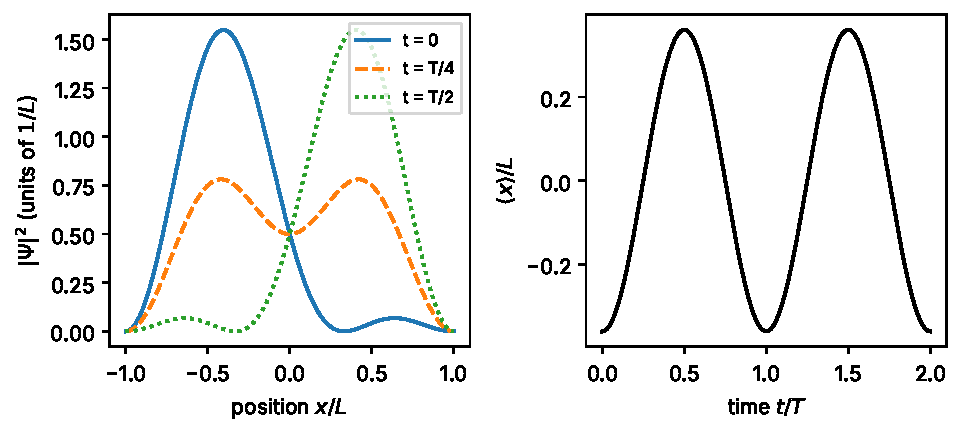
\includegraphics[width=0.85\linewidth]{figs/schrodinger_beats.pdf}
\caption{A superposition $(\psi_1e^{-iE_1t}+\psi_2e^{-iE_2t})/\sqrt2$ of the two lowest empty-box states on $[-L,L]$, units $\hbar=2m=1$ with $L=1$. Left: $\abs\Psi^2$ at $t=0$, $T/4$ and $T/2$, where $T=2\pi/(E_2-E_1)$. Right: the expectation value $\langle x\rangle$ oscillates as $\cos((E_2-E_1)t)$ with amplitude $32L/(9\pi^2)\approx0.360L$ (Problem~10 at the end of this chapter).}
\label{fig:schrodinger-beats}
\end{figure}

\begin{checkpoint}
A state is $\Psi=\frac{1}{\sqrt2}(\psi_1+\psi_2)$ at $t=0$. Someone multiplies $\psi_2$ by $-1$ (a legitimate choice of eigenfunction sign). Do the energy probabilities change? Does $\abs{\Psi}^2$ at $t=0$ change?
\end{checkpoint}
\checkanswer{The probabilities $\abs{c_n}^2=\tfrac12$ do not change. But $\abs\Psi^2$ does: the cross term $\psi_1\psi_2$ flips sign, so the probability is now piled on the other side. A sign of one eigenfunction is a convention, but a \emph{relative} sign inside a superposition is physical: $\psi_1+\psi_2$ and $\psi_1-\psi_2$ are different states.}

\begin{keyideas}
\item Expectation values: $\langle Q\rangle=\int\Psi^*\,Q\Psi\,\dd x=\bra\Psi Q\ket\Psi$; for a function $f(x)$ this is the $\abs\Psi^2$-weighted average $\int f\abs\Psi^2\dd x$.
\item Expanding $\Psi=\sum c_n\psi_n$ in orthonormal eigenfunctions gives $c_n=\braket{\psi_n}{\Psi}$, $\sum\abs{c_n}^2=1$ and $\langle H\rangle=\sum\abs{c_n}^2E_n$.
\item Energy measurements return eigenvalues $E_n$ with probabilities $\abs{c_n}^2$.
\item Observable time dependence comes only from energy differences, as beats.
\end{keyideas}

%======================================================================
\section{Hermitian operators and real eigenvalues}\label{sec:schrodinger-hermitian}
%======================================================================

\subsection{Why we need a special class of operators}

Measured energies are real numbers. If quantum mechanics is to make sense, the operator $H$ must have only real eigenvalues, and its eigenfunctions should be orthogonal so that the expansion of Sec.~\ref{sec:schrodinger-expectation} works. Recall from Chapter~\ref{ch:eigen} that a matrix with complex entries is \emph{Hermitian} if $H_{ij}=H_{ji}^*$ (equal to its conjugate transpose), and that Hermitian matrices have real eigenvalues and orthogonal eigenvectors. We now define the analogous property for operators and prove the same two results.

\subsection{Definition}

A linear operator $Q$, acting on functions that satisfy given boundary conditions, is \emph{Hermitian} if
\begin{equation}
\bra fQ\ket g=\int f^*\,(Qg)\,\dd x=\int (Qf)^*\,g\,\dd x
\label{eq:schrodinger-hermitian-def}
\end{equation}
for all such functions $f$ and $g$. In words: $Q$ may be moved from the right-hand function to the left-hand one, provided we conjugate it there. Apply Eq.~\eqref{eq:schrodinger-hermitian-def} to any two allowed functions $\psi_m,\psi_n$, for example members of an orthonormal basis. Then
\[
\bra mQ\ket n=\int(Q\psi_m)^*\psi_n\,\dd x=\left(\int\psi_n^*\,Q\psi_m\,\dd x\right)^*=\bra nQ\ket m^*,
\]
where the middle step uses $(ab)^*=a^*b^*$ inside the integral. This is the matrix condition $Q_{mn}=Q_{nm}^*$.

\subsection{The Hamiltonian with Dirichlet walls is Hermitian}

Take $H=-\frac{\hbar^2}{2m}\frac{\dd^2}{\dd x^2}+V(x)$ on $[-L,L]$ with $f(\pm L)=g(\pm L)=0$, and $V$ real. Split $H$ into its two terms.

\emph{Potential term.} $\int f^*\,Vg\,\dd x=\int (Vf)^*g\,\dd x$ requires $f^*V=(Vf)^*=V^*f^*$, true for all $f$ exactly when $V^*=V$, that is, $V$ real.

\emph{Kinetic term.} Integrate by parts twice. The first integration by parts, with $u=f^*$ and $\dd v=g''\dd x$:
\[
\int_{-L}^Lf^*g''\,\dd x=\Big[f^*g'\Big]_{-L}^L-\int_{-L}^Lf^{*\prime}g'\,\dd x=-\int_{-L}^Lf^{*\prime}g'\,\dd x,
\]
because $f^*(\pm L)=0$. The second integration by parts, with $u=f^{*\prime}$ and $\dd v=g'\dd x$ (so $v=g$):
\[
-\int_{-L}^Lf^{*\prime}g'\,\dd x=-\Big[f^{*\prime}g\Big]_{-L}^L+\int_{-L}^Lf^{*\prime\prime}g\,\dd x=\int_{-L}^Lf^{*\prime\prime}g\,\dd x,
\]
because $g(\pm L)=0$. Combining, $\int f^*g''\dd x=\int f^{*\prime\prime}g\,\dd x=\int(f'')^*g\,\dd x$; multiplying by the real constant $-\hbar^2/2m$ gives the kinetic part of Eq.~\eqref{eq:schrodinger-hermitian-def}. Adding the two parts:

\medskip
\noindent\textbf{Result.} With real $V$ and Dirichlet walls, $\bra fH\ket g=\int(Hf)^*g\,\dd x$: \emph{$H$ is Hermitian}.
\medskip

Both ingredients matter. The boundary terms vanished because of the walls, and the potential term was symmetric because $V$ is real. Change either and Hermiticity can fail.

\subsection{Two theorems}

\noindent\textbf{Theorem 1 (proved). The eigenvalues of a Hermitian operator are real.}
\emph{Proof.} Let $Q\psi=\lambda\psi$ with $\psi\neq0$. Compute $\bra\psi Q\ket\psi$ in two ways:
\begin{align*}
\int\psi^*(Q\psi)\,\dd x&=\int\psi^*\lambda\psi\,\dd x=\lambda\int\abs\psi^2\dd x,\\
\int(Q\psi)^*\psi\,\dd x&=\int\lambda^*\psi^*\psi\,\dd x=\lambda^*\int\abs\psi^2\dd x.
\end{align*}
Hermiticity says the two left sides are equal, so $(\lambda-\lambda^*)\int\abs\psi^2\dd x=0$. Since $\psi\ne0$, $\int\abs\psi^2\dd x>0$, hence $\lambda=\lambda^*$: $\lambda$ is real. $\blacksquare$

\noindent\textbf{Theorem 2 (proved). Eigenfunctions of a Hermitian operator belonging to different eigenvalues are orthogonal.}
\emph{Proof.} Let $Q\psi_m=\lambda_m\psi_m$ and $Q\psi_n=\lambda_n\psi_n$ with $\lambda_m\ne\lambda_n$. Then
\[
\int\psi_n^*(Q\psi_m)\,\dd x=\lambda_m\braket{\psi_n}{\psi_m},\qquad
\int(Q\psi_n)^*\psi_m\,\dd x=\lambda_n^*\braket{\psi_n}{\psi_m}=\lambda_n\braket{\psi_n}{\psi_m},
\]
using Theorem~1 ($\lambda_n^*=\lambda_n$) in the last step. Hermiticity equates the left sides, so $(\lambda_m-\lambda_n)\braket{\psi_n}{\psi_m}=0$, and since $\lambda_m\ne\lambda_n$, $\braket{\psi_n}{\psi_m}=0$. $\blacksquare$

These are word for word the proofs for Hermitian matrices in Chapter~\ref{ch:eigen}, with sums replaced by integrals. They justify everything in Sec.~\ref{sec:schrodinger-expectation}: real measured energies and orthonormal expansions.

\begin{beyond}
\textbf{Taken on trust: ``self-adjoint'' and completeness.} For operators on infinite-dimensional function spaces, mathematicians distinguish a \emph{Hermitian} (or \emph{symmetric}) operator, which satisfies Eq.~\eqref{eq:schrodinger-hermitian-def} on its stated domain, from a \emph{self-adjoint} one, for which the domains of the operator and its adjoint also coincide. Self-adjointness is what guarantees a full set of real eigenvalues (or, more generally, a real spectrum) and the expansion theorem: every square-integrable function can be expanded as in Eq.~\eqref{eq:schrodinger-expansion}, with the infinite sum converging in the mean-square sense. For the operators in this book ($-\dd^2/\dd x^2+V$ on a finite interval with Dirichlet walls and a bounded real $V$) both properties hold; this is part of Sturm--Liouville theory, treated in Riley, Hobson and Bence \cite{rhb}. Physicists, and the paper, often use ``Hermitian'' and ``self-adjoint'' interchangeably; we will too, except when the distinction matters (Chapter~\ref{ch:hilbert-polya}).
\end{beyond}

\subsection{Momentum is Hermitian; the plain derivative is not}

\begin{sample}{Why the $-i$ in $\hat p$ is needed}
\textbf{Problem.} On $[-L,L]$ with Dirichlet walls, show that $\hat p=-i\hbar\,\dd/\dd x$ is Hermitian but $D=\dd/\dd x$ is not.

\textbf{Step 1: integrate $D$ by parts.} For $f,g$ vanishing at $\pm L$:
\[
\int f^*g'\,\dd x=\Big[f^*g\Big]_{-L}^L-\int f^{*\prime}g\,\dd x=-\int(f')^*g\,\dd x.
\]
So $\bra fD\ket g=-\int(Df)^*g\,\dd x$: moving $D$ across costs a minus sign. The boundary term $\Big[f^*g\Big]_{-L}^L$ vanishes as soon as \emph{either} function vanishes at the walls; Problem~12 uses this. $D$ is \emph{anti}-Hermitian, not Hermitian.

\textbf{Step 2: include $-i\hbar$.} $\bra f\hat p\ket g=-i\hbar\int f^*g'\,\dd x=-i\hbar\left(-\int(f')^*g\,\dd x\right)=i\hbar\int(f')^*g\,\dd x$.

\textbf{Step 3: compare with $\int(\hat pf)^*g$.} $(\hat pf)^*=(-i\hbar f')^*=+i\hbar(f')^*$, so $\int(\hat pf)^*g\,\dd x=i\hbar\int(f')^*g\,\dd x$, the same as Step 2.

\textbf{Answer.} \[\boxed{\hat p=-i\hbar\,\tfrac{\dd}{\dd x}\ \text{is Hermitian};\quad \tfrac{\dd}{\dd x}\ \text{is anti-Hermitian}}\]
The factor $i$ converts the minus sign from integration by parts into the minus sign of complex conjugation. Without it, momentum expectation values $\bra\Psi\hat p\ket\Psi$ would not be real. (In the box, $\hat p$ has no eigenfunctions obeying the wall conditions, because $e^{ikx}$ never vanishes; its eigenfunctions $e^{ikx}$ belong to the whole line. This is one of the domain subtleties mentioned in the \texttt{beyond} box above.)
\end{sample}

\subsection{A non-Hermitian Hamiltonian has complex eigenvalues}

Return to the complex potential $V-i\Gamma/2$ with constant real $\Gamma$. If $H\psi=E\psi$ with real $E$, then
\[
\left(H-\frac{i\Gamma}2\right)\psi=E\psi-\frac{i\Gamma}2\psi=\left(E-\frac{i\Gamma}{2}\right)\psi.
\]
The eigenvalue is now the complex number $E-i\Gamma/2$. The time factor becomes $e^{-i(E-i\Gamma/2)t/\hbar}=e^{-iEt/\hbar}e^{-\Gamma t/2\hbar}$, and $\abs{\Psi}^2$ decays as $e^{-\Gamma t/\hbar}$, in agreement with Eq.~\eqref{eq:schrodinger-decay}. The real part of the energy is unchanged; only an imaginary part appears. We have found, by a two-line calculation, a fact the paper relies on in Sec.~II~E: ``a constant $iA$ shifts all eigenvalues by the same imaginary constant''. Chapter~\ref{ch:non-hermitian} develops non-Hermitian perturbations in full.

\begin{checkpoint}
Is $H=-\frac{\hbar^2}{2m}\frac{\dd^2}{\dd x^2}+V(x)-\frac{i\Gamma}{2}$, with real $V$ and constant $\Gamma\ne0$, Hermitian? What property of the eigenvalues tells you so?
\end{checkpoint}
\checkanswer{No: the potential term fails the test because $(V-i\Gamma/2)^*\ne V-i\Gamma/2$. Its eigenvalues $E-i\Gamma/2$ are not real, which by Theorem~1 is impossible for a Hermitian operator.}

\subsection{Hermiticity on a computer}

Sample a function on $N$ equally spaced interior points $x_j=-L+jh$, $j=1,\dots,N$, with spacing $h=2L/(N+1)$, so the walls sit at $x_0=-L$ and $x_{N+1}=L$ where $\psi=0$. Recall from Chapter~\ref{ch:eigen} that the second derivative $\dd^2/\dd x^2$ becomes the tridiagonal matrix with $-2/h^2$ on the diagonal and $1/h^2$ just above and below. The Hamiltonian contains $-\dd^2/\dd x^2$, so we multiply every entry by $-1$: the operator $-\dd^2/\dd x^2$ becomes the matrix with $+2/h^2$ on the diagonal and $-1/h^2$ just above and below. The potential multiplies each sample $\psi(x_j)$ by $V(x_j)$, which adds $V(x_j)$ to the $j$-th diagonal entry. So the Hamiltonian (with $\hbar^2/2m=1$) becomes the matrix
\begin{equation}
H_{jj}=\frac{2}{h^2}+V(x_j),\qquad H_{j,j\pm1}=-\frac1{h^2},\qquad\text{all other entries }0.
\label{eq:schrodinger-fd}
\end{equation}
This matrix is real and symmetric (each off-diagonal entry equals its mirror image), so it is Hermitian, and by Chapter~\ref{ch:eigen} its eigenvalues are real and its eigenvectors orthogonal. The Dirichlet walls are built in by leaving out the boundary points. A real potential is what makes the diagonal real. Chapter~\ref{ch:finite-differences} studies the accuracy of Eq.~\eqref{eq:schrodinger-fd} in detail; for now we just use it.

\begin{pycode}
import numpy as np
from scipy.linalg import eigh_tridiagonal

L, N = 44.883, 2000               # half-width of the box, interior points
h = 2*L/(N+1)                     # grid spacing
x = -L + h*np.arange(1, N+1)      # interior points
V = np.zeros(N)                   # empty box
diag = 2/h**2 + V                 # diagonal of H, Eq. (schrodinger-fd)
off = -np.ones(N-1)/h**2          # off-diagonal
E, psi = eigh_tridiagonal(diag, off, select='i', select_range=(0, 4))
exact = (np.arange(1, 6)*np.pi/(2*L))**2
print(E/exact)                    # ratios very close to 1
psi = psi/np.sqrt(np.sum(psi**2, axis=0)*h)    # normalize: sum psi^2 h = 1
print(np.sum(psi[:, 0]*psi[:, 1])*h)           # orthogonality: about 0
\end{pycode}

\begin{keyideas}
\item An operator is Hermitian if $\int f^*Qg\,\dd x=\int(Qf)^*g\,\dd x$ for all allowed $f,g$; for $H$ this needs a real potential and boundary conditions that kill the boundary terms (Dirichlet walls do).
\item Hermitian operators have real eigenvalues and orthogonal eigenfunctions (proved above, exactly as for Hermitian matrices).
\item $\hat p=-i\hbar\,\dd/\dd x$ is Hermitian; $\dd/\dd x$ alone is not.
\item A complex potential $-i\Gamma/2$ breaks Hermiticity and makes eigenvalues complex, $E-i\Gamma/2$.
\item On a grid, $H$ becomes a real symmetric tridiagonal matrix.
\end{keyideas}

%======================================================================
\section{Units with $\hbar=2m=1$}\label{sec:schrodinger-units}
% DYK-BEGIN
\begin{didyouknow}{Planck's Natural Units}
In 1899, a year before his famous quantum hypothesis, Max Planck proposed units of length, mass, time and temperature built only from fundamental constants such as $G$, $c$ and his own new constant. He argued they would keep their meaning for any civilization. Setting $\hbar=2m=1$ in this book follows the same spirit on a smaller scale: choose units so the equations carry no clutter.
\end{didyouknow}
% DYK-END
%======================================================================

\subsection{Choosing natural units}

The constants $\hbar$ and $m$ clutter every formula. Physicists remove them by choosing units adapted to the problem. Pick any length scale $\ell$ and define the energy scale
\begin{equation}
\varepsilon=\frac{\hbar^2}{2m\ell^2}.
\label{eq:schrodinger-epsilon}
\end{equation}
Measure positions in units of $\ell$ by writing $x=\ell\xi$, with $\xi$ (``xi'') a pure number. By the chain rule $\frac{\dd}{\dd x}=\frac{\dd\xi}{\dd x}\frac{\dd}{\dd\xi}=\frac1\ell\frac{\dd}{\dd\xi}$, and applying it twice, $\frac{\dd^2}{\dd x^2}=\frac1{\ell^2}\frac{\dd^2}{\dd\xi^2}$. The time-independent equation \eqref{eq:schrodinger-tise} becomes
\[
-\frac{\hbar^2}{2m\ell^2}\frac{\dd^2\psi}{\dd\xi^2}+V\psi=E\psi
\quad\Longleftrightarrow\quad
-\varepsilon\frac{\dd^2\psi}{\dd\xi^2}+V\psi=E\psi.
\]
Divide by $\varepsilon$ and define the pure numbers $\tilde V=V/\varepsilon$, $\tilde E=E/\varepsilon$:
\[
-\frac{\dd^2\psi}{\dd\xi^2}+\tilde V\psi=\tilde E\psi.
\]
Now drop the tildes and rename $\xi$ back to $x$:
\begin{equation}
\boxed{\;H=-\frac{\dd^2}{\dd x^2}+V(x),\qquad H\psi=E\psi\;}
\label{eq:schrodinger-units-H}
\end{equation}
This is the form used throughout the paper (Sec.~II~B). It is called ``units $\hbar=2m=1$'' because setting $\hbar=1$ and $m=\tfrac12$ in Eq.~\eqref{eq:schrodinger-H} gives the same thing: $\hbar^2/2m=1/(2\cdot\tfrac12)=1$. Both descriptions mean: lengths are pure numbers in units of some $\ell$, and energies are pure numbers in units of $\hbar^2/2m\ell^2$.

The time-dependent equation simplifies too. Writing $t=(\hbar/\varepsilon)\tau$, we have $\partial/\partial t=(\varepsilon/\hbar)\partial/\partial\tau$, so $i\hbar\,\partial\Psi/\partial t=i\varepsilon\,\partial\Psi/\partial\tau$, and dividing Eq.~\eqref{eq:schrodinger-tdse} by $\varepsilon$ gives $i\,\partial\Psi/\partial\tau=-\partial^2\Psi/\partial\xi^2+\tilde V\Psi$. Time is measured in units of $\hbar/\varepsilon$.

In these units some formulas become very clean:
\begin{itemize}
\item free particle: $E=k^2$ (from $E=\hbar^2k^2/2m$), so $k=\sqrt E$; and $\omega=E/\hbar=k^2$ (the right panel of \cref{fig:schrodinger-planewave});
\item particle speed $v=p/m=\hbar k/m=2k$ (from $\hbar=1$, $m=\tfrac12$);
\item empty box: $E_k=(k\pi/2L)^2$, as in Chapter~\ref{ch:eigen};
\item in a potential, the local wavenumber where $E>V(x)$ is $\sqrt{E-V(x)}$, the starting point of Chapter~\ref{ch:wkb}.
\end{itemize}

\begin{sample}{An electron in a 1 nm box, in and out of natural units}
\textbf{Problem.} (a) Find the energy unit $\varepsilon$ for an electron with $\ell=1$~nm, in eV. (b) Find the ground-state energy of an electron in an empty box of total width $1$~nm.

\textbf{Step 1: energy unit.} $\varepsilon=\hbar^2/(2m_e\ell^2)$:
\[
\varepsilon=\frac{(1.054572\times10^{-34})^2}{2(9.109384\times10^{-31})(10^{-9})^2}~\text{J}=6.104\times10^{-21}~\text{J}=0.0381~\text{eV}.
\]

\textbf{Step 2: box in natural units.} Total width $1$~nm means $2L=1$, so $L=0.5$ (in units of $\ell$). Then $E_1=(\pi/2L)^2=\pi^2=9.870$ in units of $\varepsilon$.

\textbf{Step 3: back to eV.} $E_1=9.870\times0.0381~\text{eV}=0.376$~eV.

\textbf{Answer.} \[\boxed{\varepsilon=0.0381~\text{eV},\qquad E_1=\pi^2\varepsilon=0.376~\text{eV}}\]
This agrees with the familiar SI formula $h^2/(8m_ea^2)$ for a box of width $a$, since $\frac{\hbar^2}{2m}\left(\frac{\pi}{a}\right)^2=\frac{h^2}{4\pi^2}\cdot\frac{\pi^2}{2ma^2}=\frac{h^2}{8ma^2}$.
\end{sample}

\begin{sample}{The phase of a zeta-height level}
\textbf{Problem.} In units $\hbar=2m=1$, a stationary state has energy equal to the height of the first zeta zero, $E=t_1=14.134725$ (the first of the ten zeros listed in Chapter~\ref{ch:intro}). How much time $\tau$ (in the natural time unit) does its phase factor take to rotate by $\pi$, that is, to change sign?

\textbf{Step 1:} With $\hbar=1$ the phase factor is $e^{-iE\tau}$. It equals $-1$ when $E\tau=\pi$.

\textbf{Step 2:} $\tau=\pi/E=3.141593/14.134725$.

\textbf{Answer.} \[\boxed{\tau=0.2223}\]
In the paper no particle and no physical time appear at all: only the eigenvalues matter, and they are pure numbers compared directly with the pure numbers $t_n$.
\end{sample}

\begin{checkpoint}
In units $\hbar=2m=1$, a free particle has $E=100$. What are its wavenumber and wavelength (in units of $\ell$)?
\end{checkpoint}
\checkanswer{$k=\sqrt E=10$ and $\lambda=2\pi/k=2\pi/10\approx0.628$.}

\begin{pitfall}
After switching to natural units, all numbers are pure numbers, and a formula like $E_1=(\pi/2L)^2$ only makes sense if $L$ is measured in the same unit $\ell$ used to define $\varepsilon$. Mixing a length in meters with an energy in units of $\varepsilon$ gives nonsense.
\end{pitfall}

\begin{keyideas}
\item Measuring lengths in a unit $\ell$ and energies in $\varepsilon=\hbar^2/2m\ell^2$ turns the Schr\"odinger equation into $-\psi''+V\psi=E\psi$; this is what ``units $\hbar=2m=1$'' means.
\item In these units a free particle has $k=\sqrt{E}$, $\omega=k^2$, speed $2k$; the empty box has $E_k=(k\pi/2L)^2$.
\item The paper's energies are pure numbers on the same scale as the zero heights $t_n$.
\end{keyideas}

%======================================================================
\section{Energy levels as a spectrum}\label{sec:schrodinger-spectrum}
%======================================================================

\subsection{What a spectrum is}

The \emph{spectrum} of an operator is (for the operators in this book) the set of its eigenvalues. For a particle confined by walls or by a potential that rises without bound, the spectrum is a discrete list $E_1<E_2<E_3<\cdots$ of energy levels, ordered by size and labeled by the \emph{level index} $n=1,2,\dots$. For a free particle on the whole line, every $E\ge0$ is allowed (each $k$ gives a plane wave), and the spectrum is continuous. (The plane waves are not normalizable (Problem~3), so strictly these are not eigenvalues in the sense used above. The precise notion of a continuous spectrum is beyond this book, and we do not need it: every operator in the paper lives in a box.) Confinement creates discreteness, just as pinning a string creates harmonics. \Cref{tab:schrodinger-analogy} collects the analogy.

\begin{table}[htbp]\centering
\caption{The string and the quantum particle in a box, side by side.}
\label{tab:schrodinger-analogy}
\begin{tabular}{lll}
\toprule
 & string pinned at both ends & particle in a box \\
\midrule
what waves & displacement $y(x,t)$, real & amplitude $\Psi(x,t)$, complex \\
equation & $y_{xx}=y_{tt}/v^2$ & $i\hbar\Psi_t=H\Psi$ \\
dispersion & $\omega=vk$ & $\omega=\hbar k^2/2m$ \\
boundary & $y=0$ at the ends & $\psi=0$ at the walls \\
spectrum & frequencies $f_n=nv/2\ell$ & energies $E_k=\frac{\hbar^2}{2m}(k\pi/2L)^2$ \\
observed & sound at $f_n$ & light at $(E_m-E_n)/h$ \\
\bottomrule
\end{tabular}
\end{table}

The historical spectrum is that of hydrogen. Its levels are $E_n=-13.6~\text{eV}/n^2$. We simply quote this textbook value (HRW \cite{hrw}); it comes from solving the Schr\"odinger equation in three dimensions, which this book does not do. A transition from $n=3$ to $n=2$ releases a photon of energy $13.6\left(\frac14-\frac19\right)~\text{eV}=13.6\cdot\frac5{36}~\text{eV}=1.89$~eV, and wavelength $\lambda=hc/\Delta E=(1240~\text{eV\,nm})/(1.89~\text{eV})\approx656$~nm, the red Balmer line seen in every hydrogen discharge. Measuring line positions is reading off differences of eigenvalues of $H$.

\subsection{Counting levels}

When there are many levels, a convenient summary is the \emph{counting function}
\begin{equation}
N(E)=\text{number of eigenvalues }E_n\le E.
\label{eq:schrodinger-count}
\end{equation}
It is a staircase: it jumps by one at each level and is flat in between. (The letter $N$ is also used for the number of grid points; the paper overloads it the same way, and context decides.)

For the empty box with $\hbar^2/2m=1$, $E_k=(k\pi/2L)^2\le E$ is equivalent to $k\le2L\sqrt E/\pi$, so
\begin{equation}
N_{\rm box}(E)=\left\lfloor\frac{2L\sqrt E}{\pi}\right\rfloor,
\label{eq:schrodinger-box-count}
\end{equation}
where $\lfloor y\rfloor$ (the ``floor'') is the largest integer not exceeding $y$. Dropping the floor gives a smooth curve $2L\sqrt E/\pi$. At $E=E_k$ it equals exactly $k$, where the staircase jumps up to $k$, so it touches the top corner of each step. Subtracting $\tfrac12$ gives a curve through the middle of the staircase. Either way the slope is the same. The derivative $\dd N/\dd E=L/(\pi\sqrt E)$ is the \emph{level density}, the number of levels per unit energy. The reciprocal of the density, $\pi\sqrt E/L$, is the \emph{mean spacing}. Equivalently, since the level index is $k=N$, the spacing is $\dd E/\dd k$. Differentiating $E_k=(k\pi/2L)^2$ with respect to $k$ and eliminating $k=2L\sqrt E/\pi$,
\begin{equation}
\frac{\dd E}{\dd k}=2k\left(\frac\pi{2L}\right)^2=2\cdot\frac{2L\sqrt E}{\pi}\cdot\frac{\pi^2}{4L^2}=\frac{\pi\sqrt E}{L}.
\label{eq:schrodinger-box-spacing}
\end{equation}
The empty-box levels spread \emph{apart} as $E$ grows.

\begin{sample}{Counting the paper's box}
\textbf{Problem.} For the empty box with $L=44.883$ (units $\hbar=2m=1$), how many levels lie below $E=1000$, and what is the mean spacing near $E=1000$?

\textbf{Step 1: count.} $\sqrt{1000}=31.6228$, so $2L\sqrt E/\pi=89.766\times31.6228/3.14159=903.57$. The floor is $903$.

\textbf{Step 2: spacing.} By Eq.~\eqref{eq:schrodinger-box-spacing}, $\pi\sqrt E/L=3.14159\times31.6228/44.883=2.213$.

\textbf{Answer.} \[\boxed{N_{\rm box}(1000)=903,\qquad \text{spacing}\approx2.21}\]
\end{sample}

\subsection{The zeros as a would-be spectrum}

Now compare with the zeta zeros of Chapter~\ref{ch:intro}. Their counting function $N(T)$, the number of zeros with $0<t_n\le T$, is also a staircase, and on average it follows the smooth function of paper Eq.~(1),
\begin{equation}
\Nsm(t)=\frac{t}{2\pi}\log\frac{t}{2\pi}-\frac{t}{2\pi}+\frac78,
\label{eq:schrodinger-nsm}
\end{equation}
which Chapter~\ref{ch:counting-zeros} derives ($\log$ is the natural logarithm). For instance $\Nsm(100)=29.0$, and there are exactly $29$ zeros below $100$; $\Nsm(1000)=648.6$, and there are $649$ zeros below $1000$. Differentiating Eq.~\eqref{eq:schrodinger-nsm},
\[
\frac{\dd\Nsm}{\dd t}=\frac{1}{2\pi}\log\frac{t}{2\pi}+\frac{t}{2\pi}\cdot\frac1t-\frac1{2\pi}=\frac1{2\pi}\log\frac t{2\pi},
\]
so the mean spacing near height $t$ is $2\pi/\log(t/2\pi)$, which is $1.239$ at $t=1000$ and \emph{shrinks} slowly as $t$ grows. \Cref{fig:schrodinger-staircase} shows both staircases.

Here is the first concrete hint of the program the paper tests. If the zeros were energy levels of some $H=-\dd^2/\dd x^2+V(x)$, the potential could not be the empty box: box levels spread apart with energy, while the zeros crowd together. A potential would have to be chosen so that its levels become denser at high energy. The Wu--Sprung potential is constructed (Chapter~\ref{ch:wu-sprung}) so that its semiclassical (WKB) counting function equals $\Nsm$. Its actual levels then follow the smooth zeros closely but not exactly. Whether the zeros are \emph{exactly} the spectrum of some self-adjoint operator is the Hilbert--P\'olya question (Chapter~\ref{ch:hilbert-polya}); it is an open conjecture, not a fact.

\begin{figure}[htbp]\centering
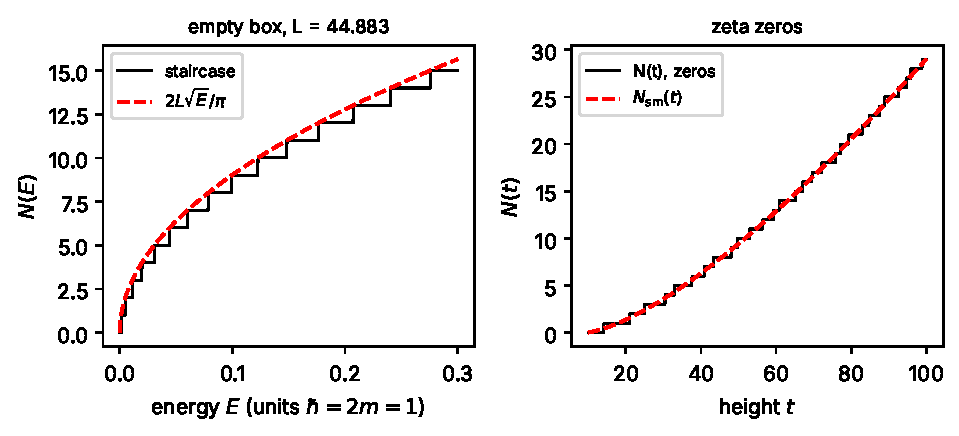
\includegraphics[width=0.85\linewidth]{figs/schrodinger_staircase.pdf}
\caption{Counting functions as staircases. Left: empty-box levels $E_k=(k\pi/2L)^2$ with $L=44.883$ (units $\hbar=2m=1$), the staircase $N_{\rm box}(E)$ and the smooth curve $2L\sqrt E/\pi$, which touches the top corner of each step (a curve through the middle would be $2L\sqrt E/\pi-\tfrac12$); the steps widen with $E$. Right: the zeta zeros, $N(t)$ (staircase) against the smooth counting function $\Nsm(t)$ of paper Eq.~(1), for $t\le100$, which runs through the middle of the steps on average (it equals $n-\tfrac12$ at the smooth zero $s_n$); the steps narrow with $t$. There are $29$ zeros below $t=100$.}
\label{fig:schrodinger-staircase}
\end{figure}

\begin{checkpoint}
A particle in an empty box of half-width $L$ and the zeta zeros both have about $650$ ``levels'' below $1000$ if $L$ is chosen suitably (what $L$?). Would the two staircases then look the same near $1000$?
\end{checkpoint}
\checkanswer{Setting $2L\sqrt{1000}/\pi\approx649$ gives $L\approx649\pi/(2\cdot31.62)\approx32$. But no: the box's spacing grows like $\sqrt E$ while the zeros' spacing shrinks like $1/\log t$, so the shapes differ even if the totals match. Matching a whole counting function requires shaping the potential.}

\begin{keyideas}
\item The spectrum of $H$ is its set of eigenvalues; confinement makes it discrete, labeled by the level index $n$.
\item The counting function $N(E)$ is a staircase; its smooth trend gives the level density and mean spacing.
\item Empty-box levels spread apart ($\dd E/\dd k=\pi\sqrt E/L$); the zeta zeros crowd together (mean spacing $2\pi/\log(t/2\pi)$). A potential must be shaped to mimic the zeros.
\end{keyideas}

%======================================================================
\section{Paper connection}\label{sec:schrodinger-paper}
%======================================================================

We now read specific sentences of the paper \cite{soniR1} with the tools of this chapter. Section, equation, table and figure numbers refer to revision R1.

\subsection{``The spectrum of a self-adjoint operator'' (Sec.~I, first sentence)}

The paper opens: ``The Hilbert--P\'olya conjecture proposes that the imaginary parts $t_n$ of the nontrivial zeros $\rho_n=\tfrac12+it_n$ of the Riemann zeta function are the spectrum of a self-adjoint operator.'' Each phrase now has content:
\begin{itemize}
\item \emph{Spectrum}: the set of eigenvalues (Sec.~\ref{sec:schrodinger-spectrum}).
\item \emph{Self-adjoint}: Hermitian in the sense of Eq.~\eqref{eq:schrodinger-hermitian-def}, with the domain subtleties of the \texttt{beyond} box in Sec.~\ref{sec:schrodinger-hermitian}.
\item \emph{Why it would matter}: by Theorem~1, a self-adjoint operator has only real eigenvalues. If every $t_n$ (defined so that the zero is $\rho_n=\tfrac12+it_n$) were such an eigenvalue, every $t_n$ would be real, which means every nontrivial zero would have real part exactly $\tfrac12$. That is the Riemann hypothesis (Chapter~\ref{ch:zeta}). The logic runs in one direction only: \emph{if} such an operator existed, RH would follow. No such operator is known; both the conjecture and RH remain open.
\end{itemize}
The paper's own fitted Hamiltonians are Hermitian by construction (real potential, Dirichlet walls), so their eigenvalues are real automatically. This says nothing about RH: the zeros the paper fits were computed numerically and are already known to lie on the critical line, and a Hermitian operator fitted to real numbers proves nothing about zeros it was not given. The paper's question (Sec.~I) is different and empirical: does such a fit \emph{predict} zeros it was not shown?

\subsection{``In units $\hbar=2m=1$, $H=-d^2/dx^2+V(x)$ with $V$ even'' (Sec.~II~B)}

This is Eq.~\eqref{eq:schrodinger-units-H}. In the paper no electron or physical length is involved: $x$ and $V$ are pure numbers (the interpolation-split paragraph of Sec.~III, where Fig.~4 is cited, says explicitly that ``$x$ and $V$ are in the units $\hbar=2m=1$ of Sec.~II~B''). The units are chosen so that the eigenvalues $E_n$ of $H$ are numbers that can be compared directly with the zero heights $t_n$; every residual in the paper, $r_n=\tilde t_n-E_n$ (Sec.~II~C), subtracts an eigenvalue from a target height. Here $\tilde t_n$ is the paper's bias-corrected target: the zero $t_n$ plus a small correction for grid error, explained in Chapter~\ref{ch:finite-differences}.

The paper's domain is $[-L,L]$ with $L=44.883$ at scale 1 and $L=59.957$ at scale 2, ``Dirichlet walls'' (Sec.~II~B), exactly the boundary conditions \eqref{eq:schrodinger-dirichlet} that make $H$ Hermitian. The potential is the Wu--Sprung potential defined by paper Eq.~(2), with bottom value $V_0=3.10073\pi\approx9.741$ at $x=0$ (Chapter~\ref{ch:wu-sprung} derives it). ``Even'' means $V(-x)=V(x)$; Chapter~\ref{ch:bound-states} explains what evenness does to the eigenfunctions. The paper solves $H\psi=E\psi$ by the finite-difference matrix of Eq.~\eqref{eq:schrodinger-fd}: ``Second-order finite differences on $N$ uniform interior points (Dirichlet walls) give a symmetric tridiagonal matrix; eigenpairs from LAPACK'' (Sec.~II~B; App.~A step 4 records the diagonal $2/dx^2+V$ and off-diagonal $-1/dx^2$, which are our $2/h^2+V_j$ and $-1/h^2$). ``Symmetric'' is the Hermiticity of Sec.~\ref{sec:schrodinger-hermitian}, and ``eigenpairs'' are the pairs $(E_n,\psi_n)$ of Sec.~\ref{sec:schrodinger-operators}.

\Cref{fig:schrodinger-wusprung} shows the Wu--Sprung potential with its lowest stationary states, computed with the matrix \eqref{eq:schrodinger-fd}. The paper reports (Sec.~II~B) that, after a grid-error correction, the levels of this potential differ from the smooth zeros $s_n$ (the solutions of $\Nsm(s_n)=n-\tfrac12$) by $0.005$ mean spacings on average and $0.063$ at worst, ``worst at low $n$''. So the unperturbed potential already reproduces the \emph{smooth} trend of the zeros; the paper's fits then try to add the fluctuations.

\begin{figure}[htbp]\centering
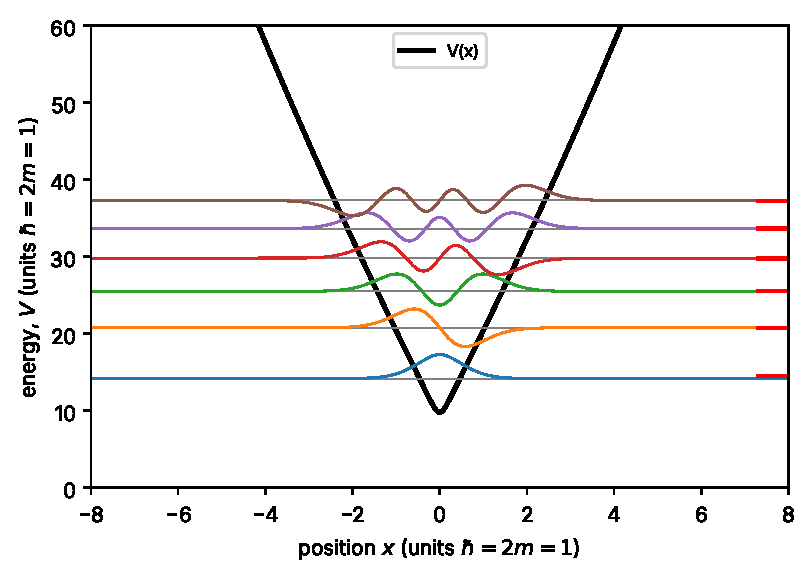
\includegraphics[width=0.85\linewidth]{figs/schrodinger_wusprung.pdf}
\caption{The Wu--Sprung potential $V(x)$ of paper Eq.~(2) (thick curve; units $\hbar=2m=1$; bottom $V_0=3.10073\pi$ at $x=0$) in the paper's scale-1 box $[-L,L]$ with $L=44.883$, of which only the central region is shown. Thin curves: the six lowest eigenfunctions $\psi_n$, normalized so that $\sum_j\psi_n(x_j)^2h=1$, drawn offset vertically to their energies $E_n$ (horizontal lines) and scaled for visibility. Even and odd states alternate, and the $n$-th state has $n-1$ nodes. Short ticks at the right edge mark the smooth zeros $s_n$, which the levels track closely.}
\label{fig:schrodinger-wusprung}
\end{figure}

The paper scores ``the first 500 levels'' at scale 1 and 1000 at scale 2 (Sec.~II~B). In App.~A step~4 it records that the scale-1 potential has $652$ states with $E\le1000$; compare $903$ for the empty box (our Sample Problem in Sec.~\ref{sec:schrodinger-spectrum}) and $\Nsm(1000)=648.6$ for the zeros. The potential is positive inside the box (it never drops below $V_0$), so at energy $E$ the local wavenumber $\sqrt{E-V(x)}$ (Sec.~\ref{sec:schrodinger-units}) is smaller than the empty-box value $\sqrt E$, and fewer half-wavelengths fit below a given $E$ (Problem~17).

\subsection{Eigenpairs and Born-rule averages (Sec.~II~C)}

The paper's fit loop (Sec.~II~C) is: ``solve for $(E_n,\psi_n)$; form residuals $r_n=\tilde t_n-E_n$ and the first-order sensitivity $A_{nk}=\int\abs{\psi_n}^2\cos(k\pi x/L)\,dx$.'' Compare with Eq.~\eqref{eq:schrodinger-favg}: $A_{nk}$ is the \emph{expectation value} of the function $\phi_k(x)=\cos(k\pi x/L)$ in the stationary state $\psi_n$,
\begin{equation}
A_{nk}=\int\abs{\psi_n}^2\phi_k\,\dd x=\bra{n}\phi_k\ket{n}=\langle\phi_k\rangle_n,
\label{eq:schrodinger-Ank}
\end{equation}
the Born-rule average of $\phi_k$ over where the particle in level $n$ is likely to be. Chapter~\ref{ch:perturbation} shows that it is exactly the first-order change of $E_n$ when the potential changes by $\phi_k$. For this to be right the eigenfunctions must be normalized; App.~A step 9 states ``$\psi$ normalized $\sum\psi^2dx=1$'', the discrete version of Eq.~\eqref{eq:schrodinger-norm} on a grid of spacing $dx=h$ (and the $\psi_n$ are real, so $\abs{\psi_n}^2=\psi_n^2$).

(The paper also uses the letter $A$ for a different object, the non-Hermitian operator of Sec.~II~E; context decides.)

\begin{sample}{The sensitivity matrix of the empty box}
\textbf{Problem.} For the empty box on $[-L,L]$, compute $A_{1k}=\int\abs{\psi_1}^2\cos(k\pi x/L)\,\dd x$ for all integers $k\ge0$, using the normalized $\psi_1$ of Eq.~\eqref{eq:schrodinger-box-states}.

\textbf{Step 1: simplify $\psi_1$.} $\sin(\pi(x+L)/2L)=\sin(\pi x/2L+\pi/2)=\cos(\pi x/2L)$, so $\abs{\psi_1}^2=\frac1L\cos^2(\pi x/2L)$.

\textbf{Step 2: double-angle formula.} $\cos^2\theta=\tfrac12(1+\cos2\theta)$ with $\theta=\pi x/2L$ gives $\abs{\psi_1}^2=\frac1{2L}\left(1+\cos(\pi x/L)\right)$.

\textbf{Step 3: integrate against $\cos(k\pi x/L)$.} 
\[
A_{1k}=\frac1{2L}\int_{-L}^{L}\cos\frac{k\pi x}{L}\,\dd x+\frac1{2L}\int_{-L}^{L}\cos\frac{\pi x}L\cos\frac{k\pi x}L\,\dd x.
\]
By the orthogonality of cosines over $[-L,L]$ (Chapter~\ref{ch:fourier-series}), the first integral is $2L$ if $k=0$ and $0$ otherwise; the second is $L$ if $k=1$ and $0$ otherwise.

\textbf{Answer.}
\[
\boxed{A_{10}=1,\qquad A_{11}=\tfrac12,\qquad A_{1k}=0\ \ (k\ge2)}
\]
$A_{10}=1$ for \emph{every} level, because $\phi_0=1$ and $\int\abs{\psi_n}^2\dd x=1$: adding a constant $c_0$ to the potential shifts every level by $c_0$. In the empty box, apart from the constant $\phi_0$, the cosine with $k=n$ affects only level $n$ (Problem~18). In the Wu--Sprung potential the eigenfunctions are no longer pure sines and each cosine reaches many levels; how that works, and why it lets the fit move levels almost independently, is the subject of Chapters~\ref{ch:perturbation} and~\ref{ch:fitting}.
\end{sample}

\subsection{Breaking Hermiticity on purpose (Secs.~II~E and~V)}

Sec.~II~E of the paper perturbs $H\to H+iA$ with $A=\sum_kc_k\phi_k$ a real function multiplying $\psi$. By Sec.~\ref{sec:schrodinger-hermitian}, the potential $V+iA$ is complex, so $H+iA$ is not Hermitian and its eigenvalues are in general complex. The ``absorptive-even'' class models ``$-i\Gamma/2$'': by Eq.~\eqref{eq:schrodinger-decay-x}, a negative imaginary potential $-i\Gamma(x)/2$ drains probability wherever $\Gamma(x)>0$, so the physical requirement is $\Gamma\ge0$, ``i.e.\ $A\le0$ pointwise'' (Sec.~II~E). The paper's safeguard (i) uses exactly the two-line calculation of Sec.~\ref{sec:schrodinger-hermitian}: ``a constant $iA$ shifts all eigenvalues by the same imaginary constant'' (and, as Chapter~\ref{ch:non-hermitian} shows, it has zero second-order real shift). Paper Eq.~(5) uses matrix elements $A_{nm}=\langle n|A|m\rangle$, which in the notation of Eq.~\eqref{eq:schrodinger-braket} means $\int\psi_n^*A\,\psi_m\,\dd x$. Finally, Sec.~V insists that ``the object of any physical claim is the exact spectrum of $H+iA$'', the set of eigenvalues of the actual (non-Hermitian) operator, not an approximation to it.

\subsection{What this chapter does not yet explain}

Why the eigenfunctions in \cref{fig:schrodinger-wusprung} have the shapes they do (Chapter~\ref{ch:bound-states}); why each level ``probes'' the potential most strongly near its classical turning points, the paper's ``position maps to level index through the classical turning point'' (Sec.~III, interpolation split; Chapter~\ref{ch:wkb}); how $V$ is built from $\Nsm$ (Chapter~\ref{ch:wu-sprung}); and how accurate the grid eigenvalues are, including the ``raw-zero null $2.09$'' of App.~A (Chapter~\ref{ch:finite-differences}).

%======================================================================
\section{Summary}\label{sec:schrodinger-summary}
%======================================================================

\begin{itemize}
\item String waves obey $\omega=vk$; pinned ends give a discrete spectrum of harmonics, Eq.~\eqref{eq:schrodinger-harmonics}.
\item De Broglie: $\lambda=h/p$, $p=\hbar k$, $E=\hbar\omega$, Eq.~\eqref{eq:schrodinger-debroglie}; a free particle has $\omega=\hbar k^2/2m$, Eq.~\eqref{eq:schrodinger-free-dispersion}.
\item The simplest linear equation with these plane-wave solutions is complex, Eq.~\eqref{eq:schrodinger-free}; adding $V$ gives the time-dependent Schr\"odinger equation \eqref{eq:schrodinger-tdse}, a postulate. Wave packets move at $v_{\rm g}=p/m$, Eq.~\eqref{eq:schrodinger-group}.
\item Separation of variables gives stationary states $\psi(x)e^{-iEt/\hbar}$ and the eigenvalue problem $H\psi=E\psi$, Eqs.~\eqref{eq:schrodinger-tise} and~\eqref{eq:schrodinger-eigen}, with $H$ of Eq.~\eqref{eq:schrodinger-H}; general solutions are superpositions, Eq.~\eqref{eq:schrodinger-general}.
\item Empty box with Dirichlet walls: $\psi_k=L^{-1/2}\sin(k\pi(x+L)/2L)$, $E_k=\frac{\hbar^2}{2m}(k\pi/2L)^2$, Eqs.~\eqref{eq:schrodinger-box-states} and~\eqref{eq:schrodinger-box-levels}.
\item Born rule: $\abs\Psi^2$ is a probability density, Eq.~\eqref{eq:schrodinger-born}; normalization \eqref{eq:schrodinger-norm} is conserved when $V$ is real, and decays as $e^{-\Gamma t/\hbar}$ for $V-i\Gamma/2$, Eq.~\eqref{eq:schrodinger-decay}.
\item Expectation values $\langle Q\rangle=\int\Psi^*Q\Psi\,\dd x$, Eq.~\eqref{eq:schrodinger-expect}; energy measurements give $E_n$ with probability $\abs{c_n}^2$, and $\langle H\rangle=\sum\abs{c_n}^2E_n$, Eq.~\eqref{eq:schrodinger-avgE}.
\item Hermitian operators, Eq.~\eqref{eq:schrodinger-hermitian-def}, have real eigenvalues and orthogonal eigenfunctions (proved); $H$ is Hermitian with real $V$ and Dirichlet walls; on a grid it is a real symmetric tridiagonal matrix, Eq.~\eqref{eq:schrodinger-fd}.
\item In units $\hbar=2m=1$, $H=-\dd^2/\dd x^2+V$, Eq.~\eqref{eq:schrodinger-units-H}; energies are pure numbers comparable with the $t_n$.
\item Counting functions are staircases; the empty box has $N(E)=\lfloor2L\sqrt E/\pi\rfloor$ and spreading levels, Eqs.~\eqref{eq:schrodinger-box-count}--\eqref{eq:schrodinger-box-spacing}; the zeros follow $\Nsm$ and crowd together.
\item The paper's sensitivity $A_{nk}$ is a Born-rule expectation value, Eq.~\eqref{eq:schrodinger-Ank}.
\end{itemize}

%======================================================================
\section{Problems}\label{sec:schrodinger-problems}
%======================================================================

Constants: $h=6.62607015\times10^{-34}$~J\,s, $\hbar=h/2\pi$, $m_e=9.1093837\times10^{-31}$~kg, $m_n=1.6749275\times10^{-27}$~kg, $1~\text{eV}=1.602176634\times10^{-19}$~J.

\begin{problemlist}

\prob{1}{Find the de Broglie wavelength of an electron with kinetic energy $10$~eV. How does it compare with the $100$~eV result of the first Sample Problem, and why?}

\prob{1}{Thermal neutrons in a reactor move at about $2200$~m/s. Find their de Broglie wavelength in nanometers.}

\prob{1}{Show that the plane wave $\Psi=e^{i(kx-\omega t)}$ has $\abs\Psi^2=1$ everywhere. Explain why it cannot be normalized on the whole line, and what that means physically.}

\prob{2}{Show in full that $\Psi=\cos(kx-\omega t)$ does not satisfy the free Schr\"odinger equation \eqref{eq:schrodinger-free} for any real $k\neq0$, by evaluating both sides at $x=0$ for two well-chosen times.}

\prob{1}{In units $\hbar=2m=1$, a free particle has $E=25$. Find its wavenumber $k$, wavelength $\lambda$, angular frequency $\omega$ and speed $v$.}

\prob{2}{Show that if $\Psi_1$ and $\Psi_2$ solve the time-independent equation $H\psi=E\psi$ with the \emph{same} $E$, then $a\Psi_1+b\Psi_2$ does too. Show by an example (two box states) that this fails if their energies differ.}

\prob{2}{In the empty box on $[-L,L]$ (units $\hbar=2m=1$), consider the trial function $\psi=A(L^2-x^2)$. (a) Show it satisfies the Dirichlet conditions. (b) Normalize it. (c) Compute $\langle H\rangle$ and compare with $E_1=\pi^2/4L^2$. Which is larger, and by what factor?}

\prob{2}{For the normalized empty-box ground state, show that $\langle x\rangle=0$ and $\langle x^2\rangle=L^2\left(\frac13-\frac2{\pi^2}\right)$. (Hint: after the substitution $u=\pi x/2L$, use $\cos^2u=\frac12(1+\cos2u)$ and integrate $u^2\cos2u$ by parts twice.)}

\prob{2}{Using the result of the box ground-state Sample Problem and symmetry, find the probability that the particle in the empty-box ground state is found in $L/2<x<L$.}

\prob{3}{For $\Psi=(\psi_1e^{-iE_1t/\hbar}+\psi_2e^{-iE_2t/\hbar})/\sqrt2$ in the empty box with real normalized $\psi_1,\psi_2$ from Eq.~\eqref{eq:schrodinger-box-states}: (a) using Eq.~\eqref{eq:schrodinger-beat}, show $\langle x\rangle(t)=I\cos((E_2-E_1)t/\hbar)$ with $I=\int x\psi_1\psi_2\,\dd x$; (b) show $\abs I=32L/(9\pi^2)$; (c) in units $\hbar=2m=1$ with $L=44.883$, find the period of the oscillation.}

\prob{3}{Repeat the norm-conservation argument of Sec.~\ref{sec:schrodinger-born} for $V-i\Gamma/2$ with constant $\Gamma>0$, showing every step, and derive Eq.~\eqref{eq:schrodinger-decay}. In units with $\hbar=1$, find the time for the norm to halve when $\Gamma=0.1$.}

\prob{2}{Show that if $V(x)$ is real and $Q=V(x)$ (a multiplication operator), then $Q$ is Hermitian for any boundary conditions. Then show that $\hat p^2=-\hbar^2\dd^2/\dd x^2$ is Hermitian by applying the momentum Sample Problem twice. (Hint: the boundary term $[f^*g]_{-L}^{L}$ in Step~1 of that Sample Problem vanishes if \emph{either} function vanishes at the walls, so the result may be used with $\hat pg$, which need not vanish there, on the right.)}

\prob{2}{Verify Theorem~2 directly for the empty box: show $\int_{-L}^{L}\psi_1\psi_2\,\dd x=0$ using a product-to-sum identity.}

\prob{2}{An electron is confined to an empty box of total width $0.2$~nm. Find its ground-state energy in eV, using natural units with $\ell=1$~nm as in the Sample Problem of Sec.~\ref{sec:schrodinger-units}.}

\prob{1}{(Paper) Sec.~II~B of the paper writes $H=-d^2/dx^2+V(x)$ without $\hbar$ or $m$. Explain why this is legitimate, and say what the numbers on the $x$ and $V$ axes of the paper's Fig.~4 mean.}

\prob{2}{(Paper) Compute the ground-state energy of the \emph{empty} box at the paper's two scales, $L=44.883$ and $L=59.957$ (units $\hbar=2m=1$). What is the ratio of the two, and why does it equal $(44.883/59.957)^2$?}

\prob{2}{(Paper) Using Eq.~\eqref{eq:schrodinger-box-count}, count the empty-box levels with $E\le1000$ for $L=44.883$. The paper (App.~A step 4) reports $652$ states with $E\le1000$ for the Wu--Sprung potential in the same box, and $\Nsm(1000)=648.6$. Explain physically why the potential reduces the count, using the local wavenumber $\sqrt{E-V(x)}$.}

\prob{2}{(Paper) For the empty box on $[-L,L]$, show that the paper's sensitivity $A_{nk}=\int\abs{\psi_n}^2\cos(k\pi x/L)\,\dd x$ equals $1$ for $k=0$, $(-1)^{n+1}/2$ for $k=n$, and $0$ otherwise. (Hint: show $\abs{\psi_n}^2=\frac1{2L}\left(1-(-1)^n\cos(n\pi x/L)\right)$.) What does this say about which basis function moves which level, to first order?}

\prob{2}{(Paper) Explain the chain of reasoning ``self-adjoint operator $\Rightarrow$ zeros on the critical line'' behind the first sentence of the paper. Then explain why the fact that the paper's fitted $H$ is Hermitian, with real eigenvalues matching many $t_n$, is \emph{not} evidence for the Riemann hypothesis.}

\prob{2}{(Paper) In the paper's absorptive-even class (Sec.~II~E), the constant basis function gives $iA=ic_0$. Using Sec.~\ref{sec:schrodinger-hermitian}, find the exact eigenvalues of $H+ic_0$ in terms of those of $H$, say what happens to the norm of a state in time for $c_0<0$, and explain why this mode cannot change any real level.}

\prob{3}{(Computational) Using numpy and \texttt{scipy.linalg.eigh\_tridiagonal}, build the matrix \eqref{eq:schrodinger-fd} for the empty box with $L=1$ and $N=500$. Compute the five lowest eigenvalues and their relative errors against $(k\pi/2)^2$. What is the relative error for $k=5$? (Chapter~\ref{ch:finite-differences} derives the exact discrete formula $\frac4{h^2}\sin^2\frac{k\pi h}{4L}$; check that it matches your numbers.)}

\prob{2}{(Computational) Using numpy, sample $\psi=e^{-\abs x}$ on a uniform grid on $[-20,20]$ with spacing $0.001$, normalize it numerically with $\sum\psi^2h=1$, and compute the probability of $\abs x<1$. Compare with the Sample Problem.}

\prob{3}{(Computational) Using \texttt{qmnt.wu\_sprung\_V} to build the potential on $N=6000$ interior points of $(-L,L)$ with $L=44.883$ (\texttt{qmnt.grid}), and \texttt{qmnt.fd\_levels} for the eigenvalues, compute the five lowest levels. Compare them with the smooth zeros \texttt{qmnt.smooth\_zeros} and express each difference in mean spacings $\gap_n=2\pi/\log(s_n/2\pi)$. Compare with the paper's reported residuals (Sec.~II~B).}

\prob{2}{(Computational) Using \texttt{qmnt.zeros} and \texttt{qmnt.Nsm}, plot the staircase $N(t)$ of the zeros and $\Nsm(t)$ for $t\le100$, and count the zeros below $t=100$.}

\prob{3}{Show that in natural units the time-dependent equation becomes $i\,\partial\Psi/\partial\tau=-\partial^2\Psi/\partial\xi^2+\tilde V\Psi$ with $t=(\hbar/\varepsilon)\tau$, and compute the time unit $\hbar/\varepsilon$ in seconds for an electron with $\ell=1$~nm.}

\prob{3}{For the normalized empty-box ground state, compute $\langle p^2\rangle$ directly from $\hat p^2=-\hbar^2\dd^2/\dd x^2$, and show $\langle H\rangle=\langle p^2\rangle/2m=E_1$. Then explain why $\langle p^2\rangle\ne\langle p\rangle^2$ (recall $\langle p\rangle=0$), and what this says about the spread of momentum.}

\prob{2}{A box state is $\Psi=\frac1{\sqrt5}(\psi_1+2i\psi_3)$. Check that it is normalized, give the probabilities of measuring $E_1$ and $E_3$, and compute $\langle H\rangle$ as a multiple of $E_1$.}

\prob{3}{Generalize the beat argument of Sec.~\ref{sec:schrodinger-tdse} to a matter wave in units $\hbar=2m=1$: superpose $e^{i(k_1x-k_1^2t)}$ and $e^{i(k_2x-k_2^2t)}$, find the exact speed of the envelope of the real part of this two-wave superposition, and show that it equals the classical speed $2k$ with $k=(k_1+k_2)/2$, with no approximation. Compare with the phase speed.}

\end{problemlist}

%======================================================================
\section{Answers to selected problems}\label{sec:schrodinger-answers}
% DYK-BEGIN
\begin{didyouknow}{Father and Son, Particle and Wave}
Louis de Broglie proposed in his 1924 thesis that electrons have wavelength $h/p$. In 1927 Clinton Davisson and Lester Germer at Bell Labs, and independently George Paget Thomson, observed electron diffraction. Davisson and Thomson shared the 1937 Nobel Prize. The twist is that G. P. Thomson's father, J. J. Thomson, had won the 1906 Nobel Prize for discovering the electron as a particle.
\end{didyouknow}
% DYK-END
%======================================================================

\textbf{1.} $K=10$~eV $=1.602\times10^{-18}$~J, $p=\sqrt{2m_eK}=1.708\times10^{-24}$~kg\,m/s, $\lambda=h/p=3.88\times10^{-10}$~m $=0.388$~nm. Since $\lambda\propto1/\sqrt K$, a tenfold drop in energy multiplies $\lambda$ by $\sqrt{10}$: $0.1226\times\sqrt{10}=0.388$~nm.

\textbf{2.} $p=m_nv=1.6749\times10^{-27}\times2200=3.685\times10^{-24}$~kg\,m/s; $\lambda=h/p=1.80\times10^{-10}$~m $=0.180$~nm, comparable to atomic spacings, which is why thermal neutrons diffract from crystals.

\textbf{3.} $\abs\Psi^2=\Psi^*\Psi=e^{-i(kx-\omega t)}e^{i(kx-\omega t)}=e^0=1$. Then $\int_{-\infty}^\infty\abs\Psi^2\dd x=\int_{-\infty}^\infty1\,\dd x$ diverges, so no constant $A$ can make $\int\abs{A\Psi}^2=1$. A plane wave is an idealization of a particle with perfectly sharp momentum spread over all space; real particles are wave packets (superpositions of plane waves) that are normalizable.

\textbf{5.} With $\hbar=2m=1$: $E=k^2$ gives $k=5$; $\lambda=2\pi/5=1.257$; $\omega=E/\hbar=25$ (equal to $k^2$); $v=p/m=\hbar k/m=5/(1/2)=10$.

\textbf{7.} (a) $L^2-x^2=0$ at $x=\pm L$. (b) $\int_{-L}^L(L^2-x^2)^2\dd x=2\int_0^L(L^4-2L^2x^2+x^4)\dd x=2\left(L^5-\tfrac23L^5+\tfrac15L^5\right)=\tfrac{16}{15}L^5$, so $A^2=15/(16L^5)$. (c) $\psi''=-2A$, so $H\psi=2A$ and $\langle H\rangle=\int A(L^2-x^2)\cdot2A\,\dd x=2A^2\left(2L^3-\tfrac23L^3\right)=\tfrac83A^2L^3=\frac{5}{2L^2}$. Since $E_1=\pi^2/4L^2=2.467/L^2$, $\langle H\rangle/E_1=10/\pi^2=1.013$: the trial function's average energy is about $1.3\%$ above the true ground state. (It can never be below $E_1$: by Eq.~\eqref{eq:schrodinger-avgE}, $\langle H\rangle=\sum\abs{c_n}^2E_n\ge E_1\sum\abs{c_n}^2=E_1$.)

\textbf{9.} The ground-state density is even, so the probabilities of $[-L,-L/2]$ and $[L/2,L]$ are equal. Together with the middle half they total $1$, so each outer quarter has $\frac12\left(1-\left(\frac12+\frac1\pi\right)\right)=\frac14-\frac1{2\pi}=0.0908$.

\textbf{11.} The extra term in $\partial\Psi/\partial t$ is $-\frac i\hbar(-\frac{i\Gamma}2)\Psi=-\frac\Gamma{2\hbar}\Psi$; in $\partial\Psi^*/\partial t$ it is $-\frac{\Gamma}{2\hbar}\Psi^*$. The kinetic terms integrate to boundary terms that vanish as before, and the real-$V$ terms cancel as before; the extra terms give $\frac{\dd P}{\dd t}=-\frac\Gamma\hbar P$, whose solution (check by differentiating) is $P(0)e^{-\Gamma t/\hbar}$. Half-life: $e^{-\Gamma t/\hbar}=\frac12$ gives $t=\hbar\ln2/\Gamma=\ln2/0.1=6.93$ (in units with $\hbar=1$).

\textbf{13.} $\psi_1\psi_2=\frac1L\sin u\sin2u$ with $u=\pi(x+L)/2L\in[0,\pi]$ and $\dd x=(2L/\pi)\dd u$. With $\sin u\sin2u=\frac12(\cos u-\cos3u)$, $\int_0^\pi\frac12(\cos u-\cos3u)\dd u=\frac12\left[\sin u-\frac{\sin3u}3\right]_0^\pi=0$.

\textbf{15.} Measuring lengths in a unit $\ell$ and energies in $\varepsilon=\hbar^2/2m\ell^2$ turns $-\frac{\hbar^2}{2m}\psi''+V\psi=E\psi$ into $-\psi''+V\psi=E\psi$ (Sec.~\ref{sec:schrodinger-units}). In the paper there is no physical particle, so $\ell$ is never specified: $x$ and $V$ on the axes of Fig.~4 are pure numbers in these units, and $V$ (like $E_n$) is on the same numerical scale as the zero heights $t_n$; for example the potential reaches $1000$ at the scale-1 wall $x=44.883$.

\textbf{17.} $2L\sqrt{1000}/\pi=903.57$, so $903$ empty-box levels lie below $1000$, against $652$ for the Wu--Sprung potential (App.~A step 4) and $\Nsm(1000)=648.6$ (there are $649$ zeros below $1000$). Inside the box the potential is positive, rising from $V_0\approx9.74$ at the center to $1000$ at the walls, so at energy $E$ the local wavenumber $\sqrt{E-V(x)}$ is smaller than the free value $\sqrt E$, and near the walls (where $V>E$) there is no oscillation at all. Fewer half-wavelengths fit, hence fewer levels below each $E$.

\textbf{19.} If $t_n$ were eigenvalues of a self-adjoint operator, Theorem~1 would make each $t_n$ real; since the zero is $\rho_n=\tfrac12+it_n$, a real $t_n$ means $\Re\rho_n=\tfrac12$ for all nontrivial zeros, which is RH. The paper's $H$ is Hermitian by construction (real $V$, Dirichlet walls), so its eigenvalues would be real whatever was fitted; the $t_n$ it fits were computed numerically and already verified to be real (on the line). Matching known real numbers with real eigenvalues adds no information about zeros not fitted, and in any case the paper finds that, for the operator families and fitting protocol it tested, the fits show no reproducible skill at predicting held-out zeros (Sec.~III). RH and the Hilbert--P\'olya conjecture remain open.

\textbf{21.} The ratios of numerical to exact eigenvalues are slightly below $1$, and the relative error grows with $k$; for $k=5$ it is $8.19\times10^{-5}$. The discrete formula gives relative error $1-\sin^2a/a^2$ with $a=k\pi h/4L=5\pi/1002$, which agrees, and is approximately $a^2/3$, growing as $k^2$. (This growth with level index is the ``dispersion'' that becomes several mean spacings at levels $401$--$500$ in the paper; Chapter~\ref{ch:finite-differences}.)

\textbf{23.} All five levels lie within $0.1$ mean spacings of $s_1,\dots,s_5$. This is consistent with the paper's statement (Sec.~II~B) that the (grid-corrected) levels of the smooth potential differ from the smooth zeros by $0.005$ spacings on average and $0.063$ at worst, with the worst cases at low $n$. A sketch of the code:
\begin{pycode}
import numpy as np, qmnt
L, N = 44.883, 6000
x = qmnt.grid(L, N)
V = np.array([qmnt.wu_sprung_V(xi) for xi in x])
E = qmnt.fd_levels(V, L, k=5)
s = np.array([qmnt.smooth_zeros(n) for n in range(1, 6)])
gap = 2*np.pi/np.log(s/(2*np.pi))
print((E - s)/gap)        # each well below 0.1 in magnitude
\end{pycode}

\textbf{25.} With $t=(\hbar/\varepsilon)\tau$, the chain rule gives $\partial/\partial t=(\varepsilon/\hbar)\partial/\partial\tau$, so $i\hbar\,\partial_t\Psi=i\varepsilon\,\partial_\tau\Psi$; with $x=\ell\xi$, $-\frac{\hbar^2}{2m}\partial_x^2=-\varepsilon\partial_\xi^2$; dividing by $\varepsilon$ gives the stated equation. For $\ell=1$~nm, $\varepsilon=6.104\times10^{-21}$~J and $\hbar/\varepsilon=1.0546\times10^{-34}/6.104\times10^{-21}~\text{s}=1.73\times10^{-14}$~s.

\textbf{27.} $\abs{1/\sqrt5}^2+\abs{2i/\sqrt5}^2=\frac15+\frac45=1$ (note $\abs{2i}^2=4$). $P(E_1)=\frac15$, $P(E_3)=\frac45$. With $E_3=9E_1$, $\langle H\rangle=\frac15E_1+\frac45\cdot9E_1=\frac{37}5E_1=7.4\,E_1$.
